% Created by tikzDevice version 0.12.3.1 on 2023-02-23 14:52:48
% !TEX encoding = UTF-8 Unicode
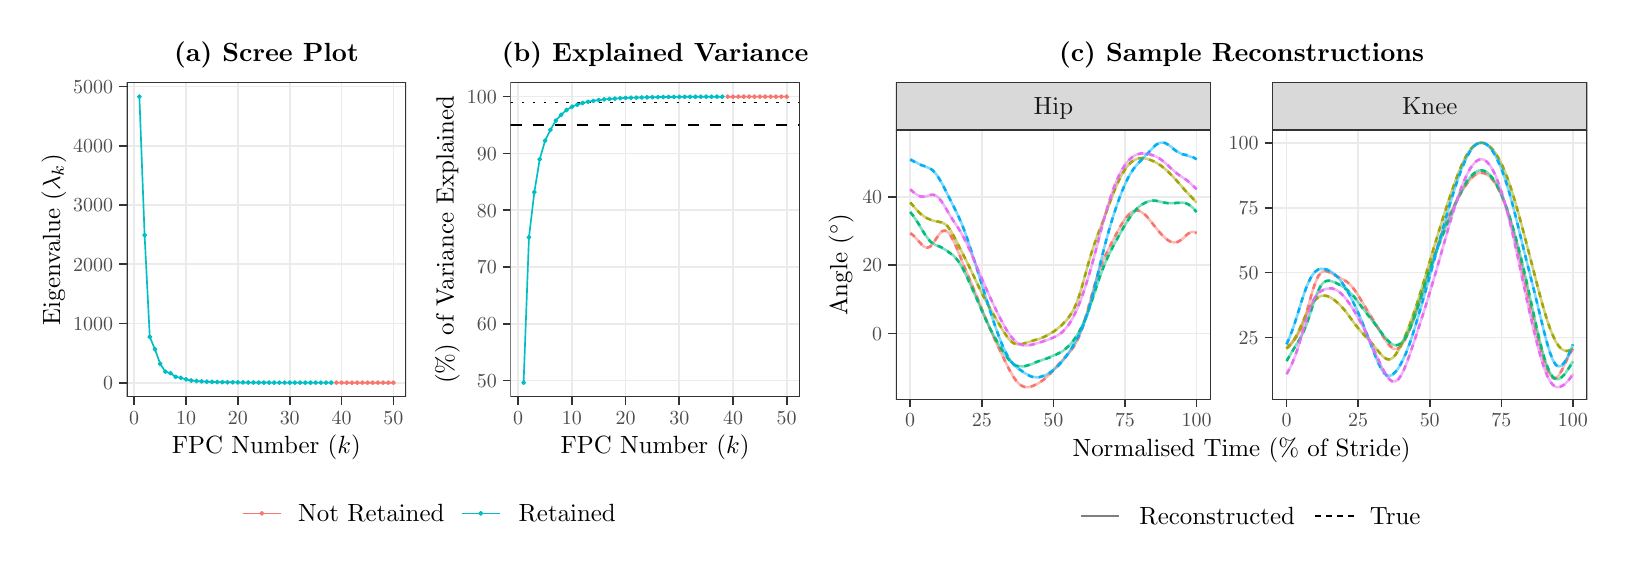
\begin{tikzpicture}[x=1pt,y=1pt]
\definecolor{fillColor}{RGB}{255,255,255}
\path[use as bounding box,fill=fillColor,fill opacity=0.00] (0,0) rectangle (569.05,189.68);
\begin{scope}
\path[clip] (  0.00, 28.34) rectangle (142.26,189.68);
\definecolor{drawColor}{RGB}{255,255,255}
\definecolor{fillColor}{RGB}{255,255,255}

\path[draw=drawColor,line width= 0.6pt,line join=round,line cap=round,fill=fillColor] (  0.00, 28.34) rectangle (142.26,189.68);
\end{scope}
\begin{scope}
\path[clip] ( 35.78, 56.24) rectangle (136.76,169.92);
\definecolor{fillColor}{RGB}{255,255,255}

\path[fill=fillColor] ( 35.78, 56.24) rectangle (136.76,169.92);
\definecolor{drawColor}{gray}{0.92}

\path[draw=drawColor,line width= 0.6pt,line join=round] ( 35.78, 61.40) --
	(136.76, 61.40);

\path[draw=drawColor,line width= 0.6pt,line join=round] ( 35.78, 82.80) --
	(136.76, 82.80);

\path[draw=drawColor,line width= 0.6pt,line join=round] ( 35.78,104.19) --
	(136.76,104.19);

\path[draw=drawColor,line width= 0.6pt,line join=round] ( 35.78,125.59) --
	(136.76,125.59);

\path[draw=drawColor,line width= 0.6pt,line join=round] ( 35.78,146.99) --
	(136.76,146.99);

\path[draw=drawColor,line width= 0.6pt,line join=round] ( 35.78,168.38) --
	(136.76,168.38);

\path[draw=drawColor,line width= 0.6pt,line join=round] ( 38.50, 56.24) --
	( 38.50,169.92);

\path[draw=drawColor,line width= 0.6pt,line join=round] ( 57.23, 56.24) --
	( 57.23,169.92);

\path[draw=drawColor,line width= 0.6pt,line join=round] ( 75.97, 56.24) --
	( 75.97,169.92);

\path[draw=drawColor,line width= 0.6pt,line join=round] ( 94.70, 56.24) --
	( 94.70,169.92);

\path[draw=drawColor,line width= 0.6pt,line join=round] (113.44, 56.24) --
	(113.44,169.92);

\path[draw=drawColor,line width= 0.6pt,line join=round] (132.17, 56.24) --
	(132.17,169.92);
\definecolor{drawColor}{RGB}{248,118,109}

\path[draw=drawColor,line width= 0.6pt,line join=round] (111.57, 61.41) --
	(113.44, 61.40) --
	(115.31, 61.40) --
	(117.19, 61.40) --
	(119.06, 61.40) --
	(120.93, 61.40) --
	(122.81, 61.40) --
	(124.68, 61.40) --
	(126.55, 61.40) --
	(128.43, 61.40) --
	(130.30, 61.40) --
	(132.17, 61.40);
\definecolor{drawColor}{RGB}{0,191,196}

\path[draw=drawColor,line width= 0.6pt,line join=round] ( 40.37,164.75) --
	( 42.25,114.73) --
	( 44.12, 77.95) --
	( 45.99, 73.47) --
	( 47.87, 68.23) --
	( 49.74, 65.38) --
	( 51.61, 64.82) --
	( 53.49, 63.51) --
	( 55.36, 63.16) --
	( 57.23, 62.59) --
	( 59.11, 62.18) --
	( 60.98, 62.01) --
	( 62.85, 61.85) --
	( 64.73, 61.76) --
	( 66.60, 61.68) --
	( 68.47, 61.64) --
	( 70.35, 61.57) --
	( 72.22, 61.55) --
	( 74.10, 61.53) --
	( 75.97, 61.50) --
	( 77.84, 61.48) --
	( 79.72, 61.46) --
	( 81.59, 61.46) --
	( 83.46, 61.45) --
	( 85.34, 61.44) --
	( 87.21, 61.43) --
	( 89.08, 61.43) --
	( 90.96, 61.43) --
	( 92.83, 61.42) --
	( 94.70, 61.42) --
	( 96.58, 61.42) --
	( 98.45, 61.41) --
	(100.32, 61.41) --
	(102.20, 61.41) --
	(104.07, 61.41) --
	(105.94, 61.41) --
	(107.82, 61.41) --
	(109.69, 61.41);
\definecolor{fillColor}{RGB}{0,191,196}

\path[draw=drawColor,line width= 0.4pt,line join=round,line cap=round,fill=fillColor] ( 40.37,164.75) circle (  0.68);

\path[draw=drawColor,line width= 0.4pt,line join=round,line cap=round,fill=fillColor] ( 42.25,114.73) circle (  0.68);

\path[draw=drawColor,line width= 0.4pt,line join=round,line cap=round,fill=fillColor] ( 44.12, 77.95) circle (  0.68);

\path[draw=drawColor,line width= 0.4pt,line join=round,line cap=round,fill=fillColor] ( 45.99, 73.47) circle (  0.68);

\path[draw=drawColor,line width= 0.4pt,line join=round,line cap=round,fill=fillColor] ( 47.87, 68.23) circle (  0.68);

\path[draw=drawColor,line width= 0.4pt,line join=round,line cap=round,fill=fillColor] ( 49.74, 65.38) circle (  0.68);

\path[draw=drawColor,line width= 0.4pt,line join=round,line cap=round,fill=fillColor] ( 51.61, 64.82) circle (  0.68);

\path[draw=drawColor,line width= 0.4pt,line join=round,line cap=round,fill=fillColor] ( 53.49, 63.51) circle (  0.68);

\path[draw=drawColor,line width= 0.4pt,line join=round,line cap=round,fill=fillColor] ( 55.36, 63.16) circle (  0.68);

\path[draw=drawColor,line width= 0.4pt,line join=round,line cap=round,fill=fillColor] ( 57.23, 62.59) circle (  0.68);

\path[draw=drawColor,line width= 0.4pt,line join=round,line cap=round,fill=fillColor] ( 59.11, 62.18) circle (  0.68);

\path[draw=drawColor,line width= 0.4pt,line join=round,line cap=round,fill=fillColor] ( 60.98, 62.01) circle (  0.68);

\path[draw=drawColor,line width= 0.4pt,line join=round,line cap=round,fill=fillColor] ( 62.85, 61.85) circle (  0.68);

\path[draw=drawColor,line width= 0.4pt,line join=round,line cap=round,fill=fillColor] ( 64.73, 61.76) circle (  0.68);

\path[draw=drawColor,line width= 0.4pt,line join=round,line cap=round,fill=fillColor] ( 66.60, 61.68) circle (  0.68);

\path[draw=drawColor,line width= 0.4pt,line join=round,line cap=round,fill=fillColor] ( 68.47, 61.64) circle (  0.68);

\path[draw=drawColor,line width= 0.4pt,line join=round,line cap=round,fill=fillColor] ( 70.35, 61.57) circle (  0.68);

\path[draw=drawColor,line width= 0.4pt,line join=round,line cap=round,fill=fillColor] ( 72.22, 61.55) circle (  0.68);

\path[draw=drawColor,line width= 0.4pt,line join=round,line cap=round,fill=fillColor] ( 74.10, 61.53) circle (  0.68);

\path[draw=drawColor,line width= 0.4pt,line join=round,line cap=round,fill=fillColor] ( 75.97, 61.50) circle (  0.68);

\path[draw=drawColor,line width= 0.4pt,line join=round,line cap=round,fill=fillColor] ( 77.84, 61.48) circle (  0.68);

\path[draw=drawColor,line width= 0.4pt,line join=round,line cap=round,fill=fillColor] ( 79.72, 61.46) circle (  0.68);

\path[draw=drawColor,line width= 0.4pt,line join=round,line cap=round,fill=fillColor] ( 81.59, 61.46) circle (  0.68);

\path[draw=drawColor,line width= 0.4pt,line join=round,line cap=round,fill=fillColor] ( 83.46, 61.45) circle (  0.68);

\path[draw=drawColor,line width= 0.4pt,line join=round,line cap=round,fill=fillColor] ( 85.34, 61.44) circle (  0.68);

\path[draw=drawColor,line width= 0.4pt,line join=round,line cap=round,fill=fillColor] ( 87.21, 61.43) circle (  0.68);

\path[draw=drawColor,line width= 0.4pt,line join=round,line cap=round,fill=fillColor] ( 89.08, 61.43) circle (  0.68);

\path[draw=drawColor,line width= 0.4pt,line join=round,line cap=round,fill=fillColor] ( 90.96, 61.43) circle (  0.68);

\path[draw=drawColor,line width= 0.4pt,line join=round,line cap=round,fill=fillColor] ( 92.83, 61.42) circle (  0.68);

\path[draw=drawColor,line width= 0.4pt,line join=round,line cap=round,fill=fillColor] ( 94.70, 61.42) circle (  0.68);

\path[draw=drawColor,line width= 0.4pt,line join=round,line cap=round,fill=fillColor] ( 96.58, 61.42) circle (  0.68);

\path[draw=drawColor,line width= 0.4pt,line join=round,line cap=round,fill=fillColor] ( 98.45, 61.41) circle (  0.68);

\path[draw=drawColor,line width= 0.4pt,line join=round,line cap=round,fill=fillColor] (100.32, 61.41) circle (  0.68);

\path[draw=drawColor,line width= 0.4pt,line join=round,line cap=round,fill=fillColor] (102.20, 61.41) circle (  0.68);

\path[draw=drawColor,line width= 0.4pt,line join=round,line cap=round,fill=fillColor] (104.07, 61.41) circle (  0.68);

\path[draw=drawColor,line width= 0.4pt,line join=round,line cap=round,fill=fillColor] (105.94, 61.41) circle (  0.68);

\path[draw=drawColor,line width= 0.4pt,line join=round,line cap=round,fill=fillColor] (107.82, 61.41) circle (  0.68);

\path[draw=drawColor,line width= 0.4pt,line join=round,line cap=round,fill=fillColor] (109.69, 61.41) circle (  0.68);
\definecolor{drawColor}{RGB}{248,118,109}
\definecolor{fillColor}{RGB}{248,118,109}

\path[draw=drawColor,line width= 0.4pt,line join=round,line cap=round,fill=fillColor] (111.57, 61.41) circle (  0.68);

\path[draw=drawColor,line width= 0.4pt,line join=round,line cap=round,fill=fillColor] (113.44, 61.40) circle (  0.68);

\path[draw=drawColor,line width= 0.4pt,line join=round,line cap=round,fill=fillColor] (115.31, 61.40) circle (  0.68);

\path[draw=drawColor,line width= 0.4pt,line join=round,line cap=round,fill=fillColor] (117.19, 61.40) circle (  0.68);

\path[draw=drawColor,line width= 0.4pt,line join=round,line cap=round,fill=fillColor] (119.06, 61.40) circle (  0.68);

\path[draw=drawColor,line width= 0.4pt,line join=round,line cap=round,fill=fillColor] (120.93, 61.40) circle (  0.68);

\path[draw=drawColor,line width= 0.4pt,line join=round,line cap=round,fill=fillColor] (122.81, 61.40) circle (  0.68);

\path[draw=drawColor,line width= 0.4pt,line join=round,line cap=round,fill=fillColor] (124.68, 61.40) circle (  0.68);

\path[draw=drawColor,line width= 0.4pt,line join=round,line cap=round,fill=fillColor] (126.55, 61.40) circle (  0.68);

\path[draw=drawColor,line width= 0.4pt,line join=round,line cap=round,fill=fillColor] (128.43, 61.40) circle (  0.68);

\path[draw=drawColor,line width= 0.4pt,line join=round,line cap=round,fill=fillColor] (130.30, 61.40) circle (  0.68);

\path[draw=drawColor,line width= 0.4pt,line join=round,line cap=round,fill=fillColor] (132.17, 61.40) circle (  0.68);
\definecolor{drawColor}{gray}{0.20}

\path[draw=drawColor,line width= 0.6pt,line join=round,line cap=round] ( 35.78, 56.24) rectangle (136.76,169.92);
\end{scope}
\begin{scope}
\path[clip] (  0.00,  0.00) rectangle (569.05,189.68);
\definecolor{drawColor}{gray}{0.30}

\node[text=drawColor,anchor=base east,inner sep=0pt, outer sep=0pt, scale=  0.72] at ( 30.83, 58.92) {0};

\node[text=drawColor,anchor=base east,inner sep=0pt, outer sep=0pt, scale=  0.72] at ( 30.83, 80.32) {1000};

\node[text=drawColor,anchor=base east,inner sep=0pt, outer sep=0pt, scale=  0.72] at ( 30.83,101.72) {2000};

\node[text=drawColor,anchor=base east,inner sep=0pt, outer sep=0pt, scale=  0.72] at ( 30.83,123.11) {3000};

\node[text=drawColor,anchor=base east,inner sep=0pt, outer sep=0pt, scale=  0.72] at ( 30.83,144.51) {4000};

\node[text=drawColor,anchor=base east,inner sep=0pt, outer sep=0pt, scale=  0.72] at ( 30.83,165.90) {5000};
\end{scope}
\begin{scope}
\path[clip] (  0.00,  0.00) rectangle (569.05,189.68);
\definecolor{drawColor}{gray}{0.20}

\path[draw=drawColor,line width= 0.6pt,line join=round] ( 33.03, 61.40) --
	( 35.78, 61.40);

\path[draw=drawColor,line width= 0.6pt,line join=round] ( 33.03, 82.80) --
	( 35.78, 82.80);

\path[draw=drawColor,line width= 0.6pt,line join=round] ( 33.03,104.19) --
	( 35.78,104.19);

\path[draw=drawColor,line width= 0.6pt,line join=round] ( 33.03,125.59) --
	( 35.78,125.59);

\path[draw=drawColor,line width= 0.6pt,line join=round] ( 33.03,146.99) --
	( 35.78,146.99);

\path[draw=drawColor,line width= 0.6pt,line join=round] ( 33.03,168.38) --
	( 35.78,168.38);
\end{scope}
\begin{scope}
\path[clip] (  0.00,  0.00) rectangle (569.05,189.68);
\definecolor{drawColor}{gray}{0.20}

\path[draw=drawColor,line width= 0.6pt,line join=round] ( 38.50, 53.49) --
	( 38.50, 56.24);

\path[draw=drawColor,line width= 0.6pt,line join=round] ( 57.23, 53.49) --
	( 57.23, 56.24);

\path[draw=drawColor,line width= 0.6pt,line join=round] ( 75.97, 53.49) --
	( 75.97, 56.24);

\path[draw=drawColor,line width= 0.6pt,line join=round] ( 94.70, 53.49) --
	( 94.70, 56.24);

\path[draw=drawColor,line width= 0.6pt,line join=round] (113.44, 53.49) --
	(113.44, 56.24);

\path[draw=drawColor,line width= 0.6pt,line join=round] (132.17, 53.49) --
	(132.17, 56.24);
\end{scope}
\begin{scope}
\path[clip] (  0.00,  0.00) rectangle (569.05,189.68);
\definecolor{drawColor}{gray}{0.30}

\node[text=drawColor,anchor=base,inner sep=0pt, outer sep=0pt, scale=  0.72] at ( 38.50, 46.33) {0};

\node[text=drawColor,anchor=base,inner sep=0pt, outer sep=0pt, scale=  0.72] at ( 57.23, 46.33) {10};

\node[text=drawColor,anchor=base,inner sep=0pt, outer sep=0pt, scale=  0.72] at ( 75.97, 46.33) {20};

\node[text=drawColor,anchor=base,inner sep=0pt, outer sep=0pt, scale=  0.72] at ( 94.70, 46.33) {30};

\node[text=drawColor,anchor=base,inner sep=0pt, outer sep=0pt, scale=  0.72] at (113.44, 46.33) {40};

\node[text=drawColor,anchor=base,inner sep=0pt, outer sep=0pt, scale=  0.72] at (132.17, 46.33) {50};
\end{scope}
\begin{scope}
\path[clip] (  0.00,  0.00) rectangle (569.05,189.68);
\definecolor{drawColor}{RGB}{0,0,0}

\node[text=drawColor,anchor=base,inner sep=0pt, outer sep=0pt, scale=  0.90] at ( 86.27, 35.83) {FPC Number ($k$)};
\end{scope}
\begin{scope}
\path[clip] (  0.00,  0.00) rectangle (569.05,189.68);
\definecolor{drawColor}{RGB}{0,0,0}

\node[text=drawColor,rotate= 90.00,anchor=base,inner sep=0pt, outer sep=0pt, scale=  0.90] at ( 11.70,113.08) {Eigenvalue ($\lambda_k$)};
\end{scope}
\begin{scope}
\path[clip] (  0.00,  0.00) rectangle (569.05,189.68);
\definecolor{drawColor}{RGB}{0,0,0}

\node[text=drawColor,anchor=base,inner sep=0pt, outer sep=0pt, scale=  0.95] at ( 86.27,177.63) {\bfseries \textbf{(a)} Scree Plot};
\end{scope}
\begin{scope}
\path[clip] (142.26, 28.34) rectangle (284.53,189.68);
\definecolor{drawColor}{RGB}{255,255,255}
\definecolor{fillColor}{RGB}{255,255,255}

\path[draw=drawColor,line width= 0.6pt,line join=round,line cap=round,fill=fillColor] (142.26, 28.34) rectangle (284.53,189.68);
\end{scope}
\begin{scope}
\path[clip] (174.45, 56.24) rectangle (279.03,169.92);
\definecolor{fillColor}{RGB}{255,255,255}

\path[fill=fillColor] (174.45, 56.24) rectangle (279.03,169.92);
\definecolor{drawColor}{gray}{0.92}

\path[draw=drawColor,line width= 0.6pt,line join=round] (174.45, 62.18) --
	(279.03, 62.18);

\path[draw=drawColor,line width= 0.6pt,line join=round] (174.45, 82.70) --
	(279.03, 82.70);

\path[draw=drawColor,line width= 0.6pt,line join=round] (174.45,103.21) --
	(279.03,103.21);

\path[draw=drawColor,line width= 0.6pt,line join=round] (174.45,123.73) --
	(279.03,123.73);

\path[draw=drawColor,line width= 0.6pt,line join=round] (174.45,144.24) --
	(279.03,144.24);

\path[draw=drawColor,line width= 0.6pt,line join=round] (174.45,164.76) --
	(279.03,164.76);

\path[draw=drawColor,line width= 0.6pt,line join=round] (177.26, 56.24) --
	(177.26,169.92);

\path[draw=drawColor,line width= 0.6pt,line join=round] (196.66, 56.24) --
	(196.66,169.92);

\path[draw=drawColor,line width= 0.6pt,line join=round] (216.07, 56.24) --
	(216.07,169.92);

\path[draw=drawColor,line width= 0.6pt,line join=round] (235.47, 56.24) --
	(235.47,169.92);

\path[draw=drawColor,line width= 0.6pt,line join=round] (254.87, 56.24) --
	(254.87,169.92);

\path[draw=drawColor,line width= 0.6pt,line join=round] (274.27, 56.24) --
	(274.27,169.92);
\definecolor{drawColor}{RGB}{0,0,0}

\path[draw=drawColor,line width= 0.6pt,dash pattern=on 4pt off 4pt ,line join=round] (174.45,154.50) -- (279.03,154.50);

\path[draw=drawColor,line width= 0.6pt,dash pattern=on 1pt off 3pt ,line join=round] (174.45,162.70) -- (279.03,162.70);
\definecolor{drawColor}{RGB}{248,118,109}

\path[draw=drawColor,line width= 0.6pt,line join=round] (252.93,164.74) --
	(254.87,164.74) --
	(256.81,164.74) --
	(258.75,164.75) --
	(260.69,164.75) --
	(262.63,164.75) --
	(264.57,164.75) --
	(266.51,164.75) --
	(268.45,164.75) --
	(270.39,164.75) --
	(272.33,164.75) --
	(274.27,164.75);
\definecolor{drawColor}{RGB}{0,191,196}

\path[draw=drawColor,line width= 0.6pt,line join=round] (179.20, 61.40) --
	(181.14,113.92) --
	(183.08,130.22) --
	(185.02,142.11) --
	(186.96,148.84) --
	(188.90,152.76) --
	(190.84,156.12) --
	(192.78,158.20) --
	(194.72,159.93) --
	(196.66,161.10) --
	(198.60,161.86) --
	(200.54,162.46) --
	(202.48,162.90) --
	(204.42,163.25) --
	(206.36,163.52) --
	(208.30,163.75) --
	(210.24,163.92) --
	(212.18,164.06) --
	(214.13,164.19) --
	(216.07,164.29) --
	(218.01,164.36) --
	(219.95,164.42) --
	(221.89,164.47) --
	(223.83,164.52) --
	(225.77,164.56) --
	(227.71,164.59) --
	(229.65,164.62) --
	(231.59,164.64) --
	(233.53,164.66) --
	(235.47,164.67) --
	(237.41,164.69) --
	(239.35,164.70) --
	(241.29,164.71) --
	(243.23,164.72) --
	(245.17,164.72) --
	(247.11,164.73) --
	(249.05,164.73) --
	(250.99,164.74);
\definecolor{fillColor}{RGB}{0,191,196}

\path[draw=drawColor,line width= 0.4pt,line join=round,line cap=round,fill=fillColor] (179.20, 61.40) circle (  0.68);

\path[draw=drawColor,line width= 0.4pt,line join=round,line cap=round,fill=fillColor] (181.14,113.92) circle (  0.68);

\path[draw=drawColor,line width= 0.4pt,line join=round,line cap=round,fill=fillColor] (183.08,130.22) circle (  0.68);

\path[draw=drawColor,line width= 0.4pt,line join=round,line cap=round,fill=fillColor] (185.02,142.11) circle (  0.68);

\path[draw=drawColor,line width= 0.4pt,line join=round,line cap=round,fill=fillColor] (186.96,148.84) circle (  0.68);

\path[draw=drawColor,line width= 0.4pt,line join=round,line cap=round,fill=fillColor] (188.90,152.76) circle (  0.68);

\path[draw=drawColor,line width= 0.4pt,line join=round,line cap=round,fill=fillColor] (190.84,156.12) circle (  0.68);

\path[draw=drawColor,line width= 0.4pt,line join=round,line cap=round,fill=fillColor] (192.78,158.20) circle (  0.68);

\path[draw=drawColor,line width= 0.4pt,line join=round,line cap=round,fill=fillColor] (194.72,159.93) circle (  0.68);

\path[draw=drawColor,line width= 0.4pt,line join=round,line cap=round,fill=fillColor] (196.66,161.10) circle (  0.68);

\path[draw=drawColor,line width= 0.4pt,line join=round,line cap=round,fill=fillColor] (198.60,161.86) circle (  0.68);

\path[draw=drawColor,line width= 0.4pt,line join=round,line cap=round,fill=fillColor] (200.54,162.46) circle (  0.68);

\path[draw=drawColor,line width= 0.4pt,line join=round,line cap=round,fill=fillColor] (202.48,162.90) circle (  0.68);

\path[draw=drawColor,line width= 0.4pt,line join=round,line cap=round,fill=fillColor] (204.42,163.25) circle (  0.68);

\path[draw=drawColor,line width= 0.4pt,line join=round,line cap=round,fill=fillColor] (206.36,163.52) circle (  0.68);

\path[draw=drawColor,line width= 0.4pt,line join=round,line cap=round,fill=fillColor] (208.30,163.75) circle (  0.68);

\path[draw=drawColor,line width= 0.4pt,line join=round,line cap=round,fill=fillColor] (210.24,163.92) circle (  0.68);

\path[draw=drawColor,line width= 0.4pt,line join=round,line cap=round,fill=fillColor] (212.18,164.06) circle (  0.68);

\path[draw=drawColor,line width= 0.4pt,line join=round,line cap=round,fill=fillColor] (214.13,164.19) circle (  0.68);

\path[draw=drawColor,line width= 0.4pt,line join=round,line cap=round,fill=fillColor] (216.07,164.29) circle (  0.68);

\path[draw=drawColor,line width= 0.4pt,line join=round,line cap=round,fill=fillColor] (218.01,164.36) circle (  0.68);

\path[draw=drawColor,line width= 0.4pt,line join=round,line cap=round,fill=fillColor] (219.95,164.42) circle (  0.68);

\path[draw=drawColor,line width= 0.4pt,line join=round,line cap=round,fill=fillColor] (221.89,164.47) circle (  0.68);

\path[draw=drawColor,line width= 0.4pt,line join=round,line cap=round,fill=fillColor] (223.83,164.52) circle (  0.68);

\path[draw=drawColor,line width= 0.4pt,line join=round,line cap=round,fill=fillColor] (225.77,164.56) circle (  0.68);

\path[draw=drawColor,line width= 0.4pt,line join=round,line cap=round,fill=fillColor] (227.71,164.59) circle (  0.68);

\path[draw=drawColor,line width= 0.4pt,line join=round,line cap=round,fill=fillColor] (229.65,164.62) circle (  0.68);

\path[draw=drawColor,line width= 0.4pt,line join=round,line cap=round,fill=fillColor] (231.59,164.64) circle (  0.68);

\path[draw=drawColor,line width= 0.4pt,line join=round,line cap=round,fill=fillColor] (233.53,164.66) circle (  0.68);

\path[draw=drawColor,line width= 0.4pt,line join=round,line cap=round,fill=fillColor] (235.47,164.67) circle (  0.68);

\path[draw=drawColor,line width= 0.4pt,line join=round,line cap=round,fill=fillColor] (237.41,164.69) circle (  0.68);

\path[draw=drawColor,line width= 0.4pt,line join=round,line cap=round,fill=fillColor] (239.35,164.70) circle (  0.68);

\path[draw=drawColor,line width= 0.4pt,line join=round,line cap=round,fill=fillColor] (241.29,164.71) circle (  0.68);

\path[draw=drawColor,line width= 0.4pt,line join=round,line cap=round,fill=fillColor] (243.23,164.72) circle (  0.68);

\path[draw=drawColor,line width= 0.4pt,line join=round,line cap=round,fill=fillColor] (245.17,164.72) circle (  0.68);

\path[draw=drawColor,line width= 0.4pt,line join=round,line cap=round,fill=fillColor] (247.11,164.73) circle (  0.68);

\path[draw=drawColor,line width= 0.4pt,line join=round,line cap=round,fill=fillColor] (249.05,164.73) circle (  0.68);

\path[draw=drawColor,line width= 0.4pt,line join=round,line cap=round,fill=fillColor] (250.99,164.74) circle (  0.68);
\definecolor{drawColor}{RGB}{248,118,109}
\definecolor{fillColor}{RGB}{248,118,109}

\path[draw=drawColor,line width= 0.4pt,line join=round,line cap=round,fill=fillColor] (252.93,164.74) circle (  0.68);

\path[draw=drawColor,line width= 0.4pt,line join=round,line cap=round,fill=fillColor] (254.87,164.74) circle (  0.68);

\path[draw=drawColor,line width= 0.4pt,line join=round,line cap=round,fill=fillColor] (256.81,164.74) circle (  0.68);

\path[draw=drawColor,line width= 0.4pt,line join=round,line cap=round,fill=fillColor] (258.75,164.75) circle (  0.68);

\path[draw=drawColor,line width= 0.4pt,line join=round,line cap=round,fill=fillColor] (260.69,164.75) circle (  0.68);

\path[draw=drawColor,line width= 0.4pt,line join=round,line cap=round,fill=fillColor] (262.63,164.75) circle (  0.68);

\path[draw=drawColor,line width= 0.4pt,line join=round,line cap=round,fill=fillColor] (264.57,164.75) circle (  0.68);

\path[draw=drawColor,line width= 0.4pt,line join=round,line cap=round,fill=fillColor] (266.51,164.75) circle (  0.68);

\path[draw=drawColor,line width= 0.4pt,line join=round,line cap=round,fill=fillColor] (268.45,164.75) circle (  0.68);

\path[draw=drawColor,line width= 0.4pt,line join=round,line cap=round,fill=fillColor] (270.39,164.75) circle (  0.68);

\path[draw=drawColor,line width= 0.4pt,line join=round,line cap=round,fill=fillColor] (272.33,164.75) circle (  0.68);

\path[draw=drawColor,line width= 0.4pt,line join=round,line cap=round,fill=fillColor] (274.27,164.75) circle (  0.68);
\definecolor{drawColor}{gray}{0.20}

\path[draw=drawColor,line width= 0.6pt,line join=round,line cap=round] (174.45, 56.24) rectangle (279.03,169.92);
\end{scope}
\begin{scope}
\path[clip] (  0.00,  0.00) rectangle (569.05,189.68);
\definecolor{drawColor}{gray}{0.30}

\node[text=drawColor,anchor=base east,inner sep=0pt, outer sep=0pt, scale=  0.72] at (169.50, 59.71) {50};

\node[text=drawColor,anchor=base east,inner sep=0pt, outer sep=0pt, scale=  0.72] at (169.50, 80.22) {60};

\node[text=drawColor,anchor=base east,inner sep=0pt, outer sep=0pt, scale=  0.72] at (169.50,100.73) {70};

\node[text=drawColor,anchor=base east,inner sep=0pt, outer sep=0pt, scale=  0.72] at (169.50,121.25) {80};

\node[text=drawColor,anchor=base east,inner sep=0pt, outer sep=0pt, scale=  0.72] at (169.50,141.76) {90};

\node[text=drawColor,anchor=base east,inner sep=0pt, outer sep=0pt, scale=  0.72] at (169.50,162.28) {100};
\end{scope}
\begin{scope}
\path[clip] (  0.00,  0.00) rectangle (569.05,189.68);
\definecolor{drawColor}{gray}{0.20}

\path[draw=drawColor,line width= 0.6pt,line join=round] (171.70, 62.18) --
	(174.45, 62.18);

\path[draw=drawColor,line width= 0.6pt,line join=round] (171.70, 82.70) --
	(174.45, 82.70);

\path[draw=drawColor,line width= 0.6pt,line join=round] (171.70,103.21) --
	(174.45,103.21);

\path[draw=drawColor,line width= 0.6pt,line join=round] (171.70,123.73) --
	(174.45,123.73);

\path[draw=drawColor,line width= 0.6pt,line join=round] (171.70,144.24) --
	(174.45,144.24);

\path[draw=drawColor,line width= 0.6pt,line join=round] (171.70,164.76) --
	(174.45,164.76);
\end{scope}
\begin{scope}
\path[clip] (  0.00,  0.00) rectangle (569.05,189.68);
\definecolor{drawColor}{gray}{0.20}

\path[draw=drawColor,line width= 0.6pt,line join=round] (177.26, 53.49) --
	(177.26, 56.24);

\path[draw=drawColor,line width= 0.6pt,line join=round] (196.66, 53.49) --
	(196.66, 56.24);

\path[draw=drawColor,line width= 0.6pt,line join=round] (216.07, 53.49) --
	(216.07, 56.24);

\path[draw=drawColor,line width= 0.6pt,line join=round] (235.47, 53.49) --
	(235.47, 56.24);

\path[draw=drawColor,line width= 0.6pt,line join=round] (254.87, 53.49) --
	(254.87, 56.24);

\path[draw=drawColor,line width= 0.6pt,line join=round] (274.27, 53.49) --
	(274.27, 56.24);
\end{scope}
\begin{scope}
\path[clip] (  0.00,  0.00) rectangle (569.05,189.68);
\definecolor{drawColor}{gray}{0.30}

\node[text=drawColor,anchor=base,inner sep=0pt, outer sep=0pt, scale=  0.72] at (177.26, 46.33) {0};

\node[text=drawColor,anchor=base,inner sep=0pt, outer sep=0pt, scale=  0.72] at (196.66, 46.33) {10};

\node[text=drawColor,anchor=base,inner sep=0pt, outer sep=0pt, scale=  0.72] at (216.07, 46.33) {20};

\node[text=drawColor,anchor=base,inner sep=0pt, outer sep=0pt, scale=  0.72] at (235.47, 46.33) {30};

\node[text=drawColor,anchor=base,inner sep=0pt, outer sep=0pt, scale=  0.72] at (254.87, 46.33) {40};

\node[text=drawColor,anchor=base,inner sep=0pt, outer sep=0pt, scale=  0.72] at (274.27, 46.33) {50};
\end{scope}
\begin{scope}
\path[clip] (  0.00,  0.00) rectangle (569.05,189.68);
\definecolor{drawColor}{RGB}{0,0,0}

\node[text=drawColor,anchor=base,inner sep=0pt, outer sep=0pt, scale=  0.90] at (226.74, 35.83) {FPC Number ($k$)};
\end{scope}
\begin{scope}
\path[clip] (  0.00,  0.00) rectangle (569.05,189.68);
\definecolor{drawColor}{RGB}{0,0,0}

\node[text=drawColor,rotate= 90.00,anchor=base,inner sep=0pt, outer sep=0pt, scale=  0.90] at (153.96,113.08) {$(\%)$ of Variance Explained};
\end{scope}
\begin{scope}
\path[clip] (  0.00,  0.00) rectangle (569.05,189.68);
\definecolor{drawColor}{RGB}{0,0,0}

\node[text=drawColor,anchor=base,inner sep=0pt, outer sep=0pt, scale=  0.95] at (226.74,177.63) {\bfseries \textbf{(b)} Explained Variance};
\end{scope}
\begin{scope}
\path[clip] (  0.00,  0.00) rectangle (569.05,189.68);
\definecolor{fillColor}{RGB}{255,255,255}

\path[fill=fillColor] ( 65.97,  0.00) rectangle (218.55, 28.34);
\end{scope}
\begin{scope}
\path[clip] (  0.00,  0.00) rectangle (569.05,189.68);
\definecolor{fillColor}{RGB}{255,255,255}

\path[fill=fillColor] ( 75.97,  5.50) rectangle ( 93.32, 22.84);
\end{scope}
\begin{scope}
\path[clip] (  0.00,  0.00) rectangle (569.05,189.68);
\definecolor{drawColor}{RGB}{248,118,109}

\path[draw=drawColor,line width= 0.6pt,line join=round] ( 77.71, 14.17) -- ( 91.58, 14.17);
\end{scope}
\begin{scope}
\path[clip] (  0.00,  0.00) rectangle (569.05,189.68);
\definecolor{drawColor}{RGB}{248,118,109}
\definecolor{fillColor}{RGB}{248,118,109}

\path[draw=drawColor,line width= 0.4pt,line join=round,line cap=round,fill=fillColor] ( 84.65, 14.17) circle (  0.68);
\end{scope}
\begin{scope}
\path[clip] (  0.00,  0.00) rectangle (569.05,189.68);
\definecolor{fillColor}{RGB}{255,255,255}

\path[fill=fillColor] (155.05,  5.50) rectangle (172.39, 22.84);
\end{scope}
\begin{scope}
\path[clip] (  0.00,  0.00) rectangle (569.05,189.68);
\definecolor{drawColor}{RGB}{0,191,196}

\path[draw=drawColor,line width= 0.6pt,line join=round] (156.78, 14.17) -- (170.66, 14.17);
\end{scope}
\begin{scope}
\path[clip] (  0.00,  0.00) rectangle (569.05,189.68);
\definecolor{drawColor}{RGB}{0,191,196}
\definecolor{fillColor}{RGB}{0,191,196}

\path[draw=drawColor,line width= 0.4pt,line join=round,line cap=round,fill=fillColor] (163.72, 14.17) circle (  0.68);
\end{scope}
\begin{scope}
\path[clip] (  0.00,  0.00) rectangle (569.05,189.68);
\definecolor{drawColor}{RGB}{0,0,0}

\node[text=drawColor,anchor=base,inner sep=0pt, outer sep=0pt, scale=  0.90] at (124.18, 11.07) {Not Retained};
\end{scope}
\begin{scope}
\path[clip] (  0.00,  0.00) rectangle (569.05,189.68);
\definecolor{drawColor}{RGB}{0,0,0}

\node[text=drawColor,anchor=base,inner sep=0pt, outer sep=0pt, scale=  0.90] at (194.97, 11.07) {Retained};
\end{scope}
\begin{scope}
\path[clip] (284.53,  0.00) rectangle (569.05,189.68);
\definecolor{drawColor}{RGB}{255,255,255}
\definecolor{fillColor}{RGB}{255,255,255}

\path[draw=drawColor,line width= 0.6pt,line join=round,line cap=round,fill=fillColor] (284.53,  0.00) rectangle (569.05,189.68);
\end{scope}
\begin{scope}
\path[clip] (313.73, 55.32) rectangle (427.56,152.65);
\definecolor{fillColor}{RGB}{255,255,255}

\path[fill=fillColor] (313.73, 55.32) rectangle (427.56,152.65);
\definecolor{drawColor}{gray}{0.92}

\path[draw=drawColor,line width= 0.6pt,line join=round] (313.73, 79.19) --
	(427.56, 79.19);

\path[draw=drawColor,line width= 0.6pt,line join=round] (313.73,103.90) --
	(427.56,103.90);

\path[draw=drawColor,line width= 0.6pt,line join=round] (313.73,128.60) --
	(427.56,128.60);

\path[draw=drawColor,line width= 0.6pt,line join=round] (318.90, 55.32) --
	(318.90,152.65);

\path[draw=drawColor,line width= 0.6pt,line join=round] (344.77, 55.32) --
	(344.77,152.65);

\path[draw=drawColor,line width= 0.6pt,line join=round] (370.64, 55.32) --
	(370.64,152.65);

\path[draw=drawColor,line width= 0.6pt,line join=round] (396.51, 55.32) --
	(396.51,152.65);

\path[draw=drawColor,line width= 0.6pt,line join=round] (422.38, 55.32) --
	(422.38,152.65);
\definecolor{drawColor}{RGB}{248,118,109}

\path[draw=drawColor,draw opacity=0.50,line width= 0.9pt,line join=round] (318.90,115.57) --
	(319.93,114.78) --
	(320.97,113.67) --
	(322.00,112.41) --
	(323.04,111.24) --
	(324.07,110.43) --
	(325.11,110.20) --
	(326.14,110.67) --
	(327.18,111.79) --
	(328.21,113.30) --
	(329.25,114.83) --
	(330.28,115.97) --
	(331.32,116.41) --
	(332.35,116.00) --
	(333.39,114.78) --
	(334.42,112.90) --
	(335.46,110.60) --
	(336.49,108.10) --
	(337.53,105.54) --
	(338.56,103.03) --
	(339.60,100.58) --
	(340.63, 98.16) --
	(341.67, 95.72) --
	(342.70, 93.21) --
	(343.74, 90.64) --
	(344.77, 88.04) --
	(345.81, 85.45) --
	(346.84, 82.93) --
	(347.87, 80.51) --
	(348.91, 78.19) --
	(349.94, 75.95) --
	(350.98, 73.77) --
	(352.01, 71.62) --
	(353.05, 69.50) --
	(354.08, 67.41) --
	(355.12, 65.43) --
	(356.15, 63.63) --
	(357.19, 62.11) --
	(358.22, 60.95) --
	(359.26, 60.19) --
	(360.29, 59.81) --
	(361.33, 59.75) --
	(362.36, 59.91) --
	(363.40, 60.26) --
	(364.43, 60.74) --
	(365.47, 61.34) --
	(366.50, 62.05) --
	(367.54, 62.89) --
	(368.57, 63.83) --
	(369.61, 64.85) --
	(370.64, 65.94) --
	(371.68, 67.07) --
	(372.71, 68.21) --
	(373.75, 69.33) --
	(374.78, 70.46) --
	(375.81, 71.62) --
	(376.85, 72.85) --
	(377.88, 74.28) --
	(378.92, 76.02) --
	(379.95, 78.22) --
	(380.99, 80.93) --
	(382.02, 84.14) --
	(383.06, 87.73) --
	(384.09, 91.52) --
	(385.13, 95.27) --
	(386.16, 98.81) --
	(387.20,101.97) --
	(388.23,104.71) --
	(389.27,107.07) --
	(390.30,109.17) --
	(391.34,111.15) --
	(392.37,113.11) --
	(393.41,115.09) --
	(394.44,117.06) --
	(395.48,118.93) --
	(396.51,120.59) --
	(397.55,121.95) --
	(398.58,122.93) --
	(399.62,123.51) --
	(400.65,123.68) --
	(401.68,123.46) --
	(402.72,122.88) --
	(403.75,122.02) --
	(404.79,120.94) --
	(405.82,119.71) --
	(406.86,118.41) --
	(407.89,117.10) --
	(408.93,115.84) --
	(409.96,114.68) --
	(411.00,113.68) --
	(412.03,112.90) --
	(413.07,112.36) --
	(414.10,112.10) --
	(415.14,112.16) --
	(416.17,112.56) --
	(417.21,113.28) --
	(418.24,114.20) --
	(419.28,115.10) --
	(420.31,115.74) --
	(421.35,115.92) --
	(422.38,115.57);
\definecolor{drawColor}{RGB}{248,118,109}

\path[draw=drawColor,line width= 0.9pt,dash pattern=on 2pt off 2pt ,line join=round] (318.90,115.38) --
	(319.93,114.65) --
	(320.97,113.64) --
	(322.00,112.48) --
	(323.04,111.35) --
	(324.07,110.48) --
	(325.11,110.16) --
	(326.14,110.57) --
	(327.18,111.71) --
	(328.21,113.32) --
	(329.25,114.92) --
	(330.28,116.05) --
	(331.32,116.41) --
	(332.35,115.92) --
	(333.39,114.69) --
	(334.42,112.89) --
	(335.46,110.67) --
	(336.49,108.19) --
	(337.53,105.61) --
	(338.56,103.03) --
	(339.60,100.52) --
	(340.63, 98.08) --
	(341.67, 95.65) --
	(342.70, 93.17) --
	(343.74, 90.63) --
	(344.77, 88.05) --
	(345.81, 85.48) --
	(346.84, 82.98) --
	(347.87, 80.58) --
	(348.91, 78.26) --
	(349.94, 76.02) --
	(350.98, 73.80) --
	(352.01, 71.60) --
	(353.05, 69.43) --
	(354.08, 67.32) --
	(355.12, 65.33) --
	(356.15, 63.56) --
	(357.19, 62.09) --
	(358.22, 60.97) --
	(359.26, 60.24) --
	(360.29, 59.86) --
	(361.33, 59.79) --
	(362.36, 59.96) --
	(363.40, 60.31) --
	(364.43, 60.78) --
	(365.47, 61.36) --
	(366.50, 62.04) --
	(367.54, 62.83) --
	(368.57, 63.73) --
	(369.61, 64.75) --
	(370.64, 65.86) --
	(371.68, 67.04) --
	(372.71, 68.24) --
	(373.75, 69.44) --
	(374.78, 70.60) --
	(375.81, 71.73) --
	(376.85, 72.90) --
	(377.88, 74.25) --
	(378.92, 75.93) --
	(379.95, 78.11) --
	(380.99, 80.86) --
	(382.02, 84.14) --
	(383.06, 87.79) --
	(384.09, 91.59) --
	(385.13, 95.32) --
	(386.16, 98.79) --
	(387.20,101.89) --
	(388.23,104.59) --
	(389.27,106.96) --
	(390.30,109.14) --
	(391.34,111.23) --
	(392.37,113.28) --
	(393.41,115.29) --
	(394.44,117.19) --
	(395.48,118.94) --
	(396.51,120.47) --
	(397.55,121.75) --
	(398.58,122.74) --
	(399.62,123.38) --
	(400.65,123.66) --
	(401.68,123.53) --
	(402.72,123.01) --
	(403.75,122.15) --
	(404.79,121.02) --
	(405.82,119.74) --
	(406.86,118.40) --
	(407.89,117.07) --
	(408.93,115.81) --
	(409.96,114.67) --
	(411.00,113.69) --
	(412.03,112.87) --
	(413.07,112.28) --
	(414.10,111.98) --
	(415.14,112.08) --
	(416.17,112.58) --
	(417.21,113.41) --
	(418.24,114.37) --
	(419.28,115.22) --
	(420.31,115.76) --
	(421.35,115.86) --
	(422.38,115.44);
\definecolor{drawColor}{RGB}{163,165,0}

\path[draw=drawColor,draw opacity=0.50,line width= 0.9pt,line join=round] (318.90,126.42) --
	(319.93,125.30) --
	(320.97,124.17) --
	(322.00,123.11) --
	(323.04,122.15) --
	(324.07,121.36) --
	(325.11,120.74) --
	(326.14,120.27) --
	(327.18,119.94) --
	(328.21,119.72) --
	(329.25,119.55) --
	(330.28,119.31) --
	(331.32,118.82) --
	(332.35,117.93) --
	(333.39,116.57) --
	(334.42,114.82) --
	(335.46,112.83) --
	(336.49,110.75) --
	(337.53,108.69) --
	(338.56,106.65) --
	(339.60,104.60) --
	(340.63,102.49) --
	(341.67,100.30) --
	(342.70, 98.08) --
	(343.74, 95.90) --
	(344.77, 93.80) --
	(345.81, 91.80) --
	(346.84, 89.90) --
	(347.87, 88.05) --
	(348.91, 86.24) --
	(349.94, 84.44) --
	(350.98, 82.64) --
	(352.01, 80.87) --
	(353.05, 79.21) --
	(354.08, 77.75) --
	(355.12, 76.57) --
	(356.15, 75.76) --
	(357.19, 75.33) --
	(358.22, 75.24) --
	(359.26, 75.39) --
	(360.29, 75.67) --
	(361.33, 75.98) --
	(362.36, 76.29) --
	(363.40, 76.57) --
	(364.43, 76.87) --
	(365.47, 77.21) --
	(366.50, 77.61) --
	(367.54, 78.08) --
	(368.57, 78.62) --
	(369.61, 79.22) --
	(370.64, 79.88) --
	(371.68, 80.59) --
	(372.71, 81.38) --
	(373.75, 82.27) --
	(374.78, 83.27) --
	(375.81, 84.46) --
	(376.85, 85.90) --
	(377.88, 87.70) --
	(378.92, 89.99) --
	(379.95, 92.84) --
	(380.99, 96.20) --
	(382.02, 99.91) --
	(383.06,103.68) --
	(384.09,107.26) --
	(385.13,110.53) --
	(386.16,113.49) --
	(387.20,116.26) --
	(388.23,118.96) --
	(389.27,121.69) --
	(390.30,124.47) --
	(391.34,127.25) --
	(392.37,129.95) --
	(393.41,132.48) --
	(394.44,134.77) --
	(395.48,136.78) --
	(396.51,138.47) --
	(397.55,139.85) --
	(398.58,140.92) --
	(399.62,141.69) --
	(400.65,142.19) --
	(401.68,142.46) --
	(402.72,142.52) --
	(403.75,142.41) --
	(404.79,142.17) --
	(405.82,141.82) --
	(406.86,141.38) --
	(407.89,140.84) --
	(408.93,140.20) --
	(409.96,139.47) --
	(411.00,138.62) --
	(412.03,137.69) --
	(413.07,136.67) --
	(414.10,135.58) --
	(415.14,134.44) --
	(416.17,133.26) --
	(417.21,132.08) --
	(418.24,130.92) --
	(419.28,129.79) --
	(420.31,128.68) --
	(421.35,127.57) --
	(422.38,126.44);
\definecolor{drawColor}{RGB}{163,165,0}

\path[draw=drawColor,line width= 0.9pt,dash pattern=on 2pt off 2pt ,line join=round] (318.90,126.54) --
	(319.93,125.40) --
	(320.97,124.19) --
	(322.00,123.02) --
	(323.04,122.02) --
	(324.07,121.28) --
	(325.11,120.75) --
	(326.14,120.35) --
	(327.18,120.00) --
	(328.21,119.72) --
	(329.25,119.52) --
	(330.28,119.29) --
	(331.32,118.84) --
	(332.35,117.96) --
	(333.39,116.60) --
	(334.42,114.82) --
	(335.46,112.81) --
	(336.49,110.73) --
	(337.53,108.68) --
	(338.56,106.65) --
	(339.60,104.60) --
	(340.63,102.48) --
	(341.67,100.30) --
	(342.70, 98.09) --
	(343.74, 95.91) --
	(344.77, 93.81) --
	(345.81, 91.80) --
	(346.84, 89.87) --
	(347.87, 88.01) --
	(348.91, 86.20) --
	(349.94, 84.43) --
	(350.98, 82.67) --
	(352.01, 80.95) --
	(353.05, 79.29) --
	(354.08, 77.79) --
	(355.12, 76.57) --
	(356.15, 75.71) --
	(357.19, 75.25) --
	(358.22, 75.16) --
	(359.26, 75.33) --
	(360.29, 75.65) --
	(361.33, 76.01) --
	(362.36, 76.34) --
	(363.40, 76.65) --
	(364.43, 76.95) --
	(365.47, 77.27) --
	(366.50, 77.63) --
	(367.54, 78.06) --
	(368.57, 78.56) --
	(369.61, 79.13) --
	(370.64, 79.78) --
	(371.68, 80.52) --
	(372.71, 81.36) --
	(373.75, 82.31) --
	(374.78, 83.38) --
	(375.81, 84.59) --
	(376.85, 86.00) --
	(377.88, 87.72) --
	(378.92, 89.92) --
	(379.95, 92.72) --
	(380.99, 96.11) --
	(382.02, 99.89) --
	(383.06,103.73) --
	(384.09,107.34) --
	(385.13,110.58) --
	(386.16,113.47) --
	(387.20,116.18) --
	(388.23,118.88) --
	(389.27,121.66) --
	(390.30,124.51) --
	(391.34,127.35) --
	(392.37,130.06) --
	(393.41,132.54) --
	(394.44,134.76) --
	(395.48,136.70) --
	(396.51,138.37) --
	(397.55,139.77) --
	(398.58,140.88) --
	(399.62,141.71) --
	(400.65,142.24) --
	(401.68,142.50) --
	(402.72,142.54) --
	(403.75,142.41) --
	(404.79,142.17) --
	(405.82,141.83) --
	(406.86,141.40) --
	(407.89,140.86) --
	(408.93,140.21) --
	(409.96,139.45) --
	(411.00,138.59) --
	(412.03,137.65) --
	(413.07,136.64) --
	(414.10,135.58) --
	(415.14,134.47) --
	(416.17,133.29) --
	(417.21,132.07) --
	(418.24,130.86) --
	(419.28,129.72) --
	(420.31,128.66) --
	(421.35,127.63) --
	(422.38,126.53);
\definecolor{drawColor}{RGB}{0,191,125}

\path[draw=drawColor,draw opacity=0.50,line width= 0.9pt,line join=round] (318.90,123.12) --
	(319.93,121.76) --
	(320.97,120.23) --
	(322.00,118.58) --
	(323.04,116.89) --
	(324.07,115.23) --
	(325.11,113.75) --
	(326.14,112.55) --
	(327.18,111.68) --
	(328.21,111.08) --
	(329.25,110.61) --
	(330.28,110.13) --
	(331.32,109.58) --
	(332.35,108.96) --
	(333.39,108.26) --
	(334.42,107.41) --
	(335.46,106.34) --
	(336.49,104.97) --
	(337.53,103.28) --
	(338.56,101.32) --
	(339.60, 99.16) --
	(340.63, 96.89) --
	(341.67, 94.56) --
	(342.70, 92.21) --
	(343.74, 89.86) --
	(344.77, 87.52) --
	(345.81, 85.21) --
	(346.84, 82.97) --
	(347.87, 80.81) --
	(348.91, 78.74) --
	(349.94, 76.78) --
	(350.98, 74.94) --
	(352.01, 73.22) --
	(353.05, 71.66) --
	(354.08, 70.28) --
	(355.12, 69.13) --
	(356.15, 68.25) --
	(357.19, 67.65) --
	(358.22, 67.33) --
	(359.26, 67.25) --
	(360.29, 67.37) --
	(361.33, 67.62) --
	(362.36, 67.94) --
	(363.40, 68.32) --
	(364.43, 68.72) --
	(365.47, 69.12) --
	(366.50, 69.54) --
	(367.54, 69.96) --
	(368.57, 70.37) --
	(369.61, 70.77) --
	(370.64, 71.17) --
	(371.68, 71.60) --
	(372.71, 72.08) --
	(373.75, 72.65) --
	(374.78, 73.37) --
	(375.81, 74.25) --
	(376.85, 75.34) --
	(377.88, 76.63) --
	(378.92, 78.12) --
	(379.95, 79.85) --
	(380.99, 81.85) --
	(382.02, 84.15) --
	(383.06, 86.75) --
	(384.09, 89.64) --
	(385.13, 92.72) --
	(386.16, 95.88) --
	(387.20, 98.97) --
	(388.23,101.86) --
	(389.27,104.48) --
	(390.30,106.82) --
	(391.34,108.95) --
	(392.37,110.95) --
	(393.41,112.86) --
	(394.44,114.73) --
	(395.48,116.56) --
	(396.51,118.34) --
	(397.55,120.01) --
	(398.58,121.55) --
	(399.62,122.91) --
	(400.65,124.09) --
	(401.68,125.06) --
	(402.72,125.85) --
	(403.75,126.45) --
	(404.79,126.87) --
	(405.82,127.10) --
	(406.86,127.15) --
	(407.89,127.05) --
	(408.93,126.86) --
	(409.96,126.63) --
	(411.00,126.43) --
	(412.03,126.29) --
	(413.07,126.24) --
	(414.10,126.26) --
	(415.14,126.34) --
	(416.17,126.44) --
	(417.21,126.46) --
	(418.24,126.32) --
	(419.28,125.92) --
	(420.31,125.24) --
	(421.35,124.27) --
	(422.38,123.07);
\definecolor{drawColor}{RGB}{0,191,125}

\path[draw=drawColor,line width= 0.9pt,dash pattern=on 2pt off 2pt ,line join=round] (318.90,123.06) --
	(319.93,121.80) --
	(320.97,120.34) --
	(322.00,118.70) --
	(323.04,116.95) --
	(324.07,115.19) --
	(325.11,113.63) --
	(326.14,112.42) --
	(327.18,111.60) --
	(328.21,111.10) --
	(329.25,110.72) --
	(330.28,110.27) --
	(331.32,109.65) --
	(332.35,108.90) --
	(333.39,108.12) --
	(334.42,107.31) --
	(335.46,106.34) --
	(336.49,105.06) --
	(337.53,103.38) --
	(338.56,101.36) --
	(339.60, 99.15) --
	(340.63, 96.88) --
	(341.67, 94.59) --
	(342.70, 92.24) --
	(343.74, 89.83) --
	(344.77, 87.41) --
	(345.81, 85.05) --
	(346.84, 82.82) --
	(347.87, 80.74) --
	(348.91, 78.80) --
	(349.94, 76.95) --
	(350.98, 75.15) --
	(352.01, 73.40) --
	(353.05, 71.75) --
	(354.08, 70.26) --
	(355.12, 69.03) --
	(356.15, 68.10) --
	(357.19, 67.50) --
	(358.22, 67.21) --
	(359.26, 67.18) --
	(360.29, 67.35) --
	(361.33, 67.66) --
	(362.36, 68.06) --
	(363.40, 68.48) --
	(364.43, 68.88) --
	(365.47, 69.24) --
	(366.50, 69.55) --
	(367.54, 69.87) --
	(368.57, 70.21) --
	(369.61, 70.60) --
	(370.64, 71.05) --
	(371.68, 71.56) --
	(372.71, 72.11) --
	(373.75, 72.74) --
	(374.78, 73.46) --
	(375.81, 74.34) --
	(376.85, 75.39) --
	(377.88, 76.65) --
	(378.92, 78.12) --
	(379.95, 79.82) --
	(380.99, 81.77) --
	(382.02, 84.06) --
	(383.06, 86.70) --
	(384.09, 89.65) --
	(385.13, 92.78) --
	(386.16, 95.95) --
	(387.20, 99.01) --
	(388.23,101.86) --
	(389.27,104.46) --
	(390.30,106.79) --
	(391.34,108.91) --
	(392.37,110.91) --
	(393.41,112.84) --
	(394.44,114.75) --
	(395.48,116.61) --
	(396.51,118.39) --
	(397.55,120.05) --
	(398.58,121.57) --
	(399.62,122.92) --
	(400.65,124.08) --
	(401.68,125.03) --
	(402.72,125.79) --
	(403.75,126.37) --
	(404.79,126.81) --
	(405.82,127.10) --
	(406.86,127.21) --
	(407.89,127.13) --
	(408.93,126.91) --
	(409.96,126.63) --
	(411.00,126.40) --
	(412.03,126.28) --
	(413.07,126.26) --
	(414.10,126.29) --
	(415.14,126.34) --
	(416.17,126.41) --
	(417.21,126.43) --
	(418.24,126.29) --
	(419.28,125.88) --
	(420.31,125.20) --
	(421.35,124.26) --
	(422.38,123.07);
\definecolor{drawColor}{RGB}{0,176,246}

\path[draw=drawColor,draw opacity=0.50,line width= 0.9pt,line join=round] (318.90,142.17) --
	(319.93,141.67) --
	(320.97,141.07) --
	(322.00,140.47) --
	(323.04,139.96) --
	(324.07,139.56) --
	(325.11,139.20) --
	(326.14,138.72) --
	(327.18,137.97) --
	(328.21,136.87) --
	(329.25,135.39) --
	(330.28,133.60) --
	(331.32,131.60) --
	(332.35,129.49) --
	(333.39,127.41) --
	(334.42,125.38) --
	(335.46,123.34) --
	(336.49,121.19) --
	(337.53,118.80) --
	(338.56,116.14) --
	(339.60,113.20) --
	(340.63,110.07) --
	(341.67,106.82) --
	(342.70,103.51) --
	(343.74,100.19) --
	(344.77, 96.87) --
	(345.81, 93.58) --
	(346.84, 90.30) --
	(347.87, 87.06) --
	(348.91, 83.89) --
	(349.94, 80.85) --
	(350.98, 77.99) --
	(352.01, 75.37) --
	(353.05, 73.05) --
	(354.08, 71.06) --
	(355.12, 69.42) --
	(356.15, 68.11) --
	(357.19, 67.07) --
	(358.22, 66.23) --
	(359.26, 65.51) --
	(360.29, 64.86) --
	(361.33, 64.29) --
	(362.36, 63.81) --
	(363.40, 63.48) --
	(364.43, 63.32) --
	(365.47, 63.35) --
	(366.50, 63.58) --
	(367.54, 63.99) --
	(368.57, 64.55) --
	(369.61, 65.23) --
	(370.64, 66.02) --
	(371.68, 66.90) --
	(372.71, 67.89) --
	(373.75, 68.99) --
	(374.78, 70.24) --
	(375.81, 71.66) --
	(376.85, 73.24) --
	(377.88, 74.96) --
	(378.92, 76.82) --
	(379.95, 78.81) --
	(380.99, 81.03) --
	(382.02, 83.61) --
	(383.06, 86.65) --
	(384.09, 90.22) --
	(385.13, 94.23) --
	(386.16, 98.51) --
	(387.20,102.86) --
	(388.23,107.12) --
	(389.27,111.18) --
	(390.30,114.99) --
	(391.34,118.56) --
	(392.37,121.91) --
	(393.41,125.04) --
	(394.44,127.97) --
	(395.48,130.67) --
	(396.51,133.10) --
	(397.55,135.24) --
	(398.58,137.09) --
	(399.62,138.65) --
	(400.65,139.98) --
	(401.68,141.14) --
	(402.72,142.20) --
	(403.75,143.25) --
	(404.79,144.34) --
	(405.82,145.45) --
	(406.86,146.52) --
	(407.89,147.41) --
	(408.93,147.99) --
	(409.96,148.19) --
	(411.00,147.99) --
	(412.03,147.46) --
	(413.07,146.72) --
	(414.10,145.90) --
	(415.14,145.12) --
	(416.17,144.46) --
	(417.21,143.96) --
	(418.24,143.61) --
	(419.28,143.33) --
	(420.31,143.05) --
	(421.35,142.68) --
	(422.38,142.18);
\definecolor{drawColor}{RGB}{0,176,246}

\path[draw=drawColor,line width= 0.9pt,dash pattern=on 2pt off 2pt ,line join=round] (318.90,142.03) --
	(319.93,141.43) --
	(320.97,140.86) --
	(322.00,140.37) --
	(323.04,139.98) --
	(324.07,139.68) --
	(325.11,139.34) --
	(326.14,138.81) --
	(327.18,137.99) --
	(328.21,136.81) --
	(329.25,135.30) --
	(330.28,133.52) --
	(331.32,131.57) --
	(332.35,129.53) --
	(333.39,127.48) --
	(334.42,125.43) --
	(335.46,123.35) --
	(336.49,121.17) --
	(337.53,118.77) --
	(338.56,116.11) --
	(339.60,113.19) --
	(340.63,110.06) --
	(341.67,106.82) --
	(342.70,103.53) --
	(343.74,100.23) --
	(344.77, 96.92) --
	(345.81, 93.59) --
	(346.84, 90.29) --
	(347.87, 87.03) --
	(348.91, 83.87) --
	(349.94, 80.85) --
	(350.98, 78.01) --
	(352.01, 75.38) --
	(353.05, 73.03) --
	(354.08, 71.00) --
	(355.12, 69.35) --
	(356.15, 68.08) --
	(357.19, 67.12) --
	(358.22, 66.34) --
	(359.26, 65.62) --
	(360.29, 64.91) --
	(361.33, 64.24) --
	(362.36, 63.71) --
	(363.40, 63.38) --
	(364.43, 63.28) --
	(365.47, 63.40) --
	(366.50, 63.67) --
	(367.54, 64.07) --
	(368.57, 64.58) --
	(369.61, 65.19) --
	(370.64, 65.93) --
	(371.68, 66.81) --
	(372.71, 67.83) --
	(373.75, 69.01) --
	(374.78, 70.32) --
	(375.81, 71.75) --
	(376.85, 73.29) --
	(377.88, 74.94) --
	(378.92, 76.73) --
	(379.95, 78.73) --
	(380.99, 81.01) --
	(382.02, 83.66) --
	(383.06, 86.74) --
	(384.09, 90.27) --
	(385.13, 94.21) --
	(386.16, 98.44) --
	(387.20,102.78) --
	(388.23,107.07) --
	(389.27,111.17) --
	(390.30,115.02) --
	(391.34,118.60) --
	(392.37,121.93) --
	(393.41,125.05) --
	(394.44,127.97) --
	(395.48,130.66) --
	(396.51,133.10) --
	(397.55,135.26) --
	(398.58,137.12) --
	(399.62,138.69) --
	(400.65,139.99) --
	(401.68,141.10) --
	(402.72,142.13) --
	(403.75,143.16) --
	(404.79,144.28) --
	(405.82,145.47) --
	(406.86,146.60) --
	(407.89,147.50) --
	(408.93,148.06) --
	(409.96,148.22) --
	(411.00,148.01) --
	(412.03,147.46) --
	(413.07,146.67) --
	(414.10,145.78) --
	(415.14,144.95) --
	(416.17,144.32) --
	(417.21,143.95) --
	(418.24,143.78) --
	(419.28,143.61) --
	(420.31,143.29) --
	(421.35,142.76) --
	(422.38,142.07);
\definecolor{drawColor}{RGB}{231,107,243}

\path[draw=drawColor,draw opacity=0.50,line width= 0.9pt,line join=round] (318.90,131.28) --
	(319.93,130.38) --
	(320.97,129.56) --
	(322.00,128.94) --
	(323.04,128.61) --
	(324.07,128.61) --
	(325.11,128.88) --
	(326.14,129.21) --
	(327.18,129.33) --
	(328.21,129.01) --
	(329.25,128.15) --
	(330.28,126.81) --
	(331.32,125.16) --
	(332.35,123.40) --
	(333.39,121.68) --
	(334.42,120.06) --
	(335.46,118.50) --
	(336.49,116.90) --
	(337.53,115.17) --
	(338.56,113.23) --
	(339.60,111.10) --
	(340.63,108.79) --
	(341.67,106.38) --
	(342.70,103.93) --
	(343.74,101.47) --
	(344.77, 99.04) --
	(345.81, 96.64) --
	(346.84, 94.30) --
	(347.87, 92.01) --
	(348.91, 89.78) --
	(349.94, 87.62) --
	(350.98, 85.53) --
	(352.01, 83.53) --
	(353.05, 81.64) --
	(354.08, 79.90) --
	(355.12, 78.36) --
	(356.15, 77.08) --
	(357.19, 76.09) --
	(358.22, 75.41) --
	(359.26, 75.00) --
	(360.29, 74.85) --
	(361.33, 74.88) --
	(362.36, 75.05) --
	(363.40, 75.29) --
	(364.43, 75.58) --
	(365.47, 75.88) --
	(366.50, 76.19) --
	(367.54, 76.52) --
	(368.57, 76.86) --
	(369.61, 77.24) --
	(370.64, 77.67) --
	(371.68, 78.19) --
	(372.71, 78.83) --
	(373.75, 79.65) --
	(374.78, 80.66) --
	(375.81, 81.91) --
	(376.85, 83.41) --
	(377.88, 85.20) --
	(378.92, 87.33) --
	(379.95, 89.79) --
	(380.99, 92.56) --
	(382.02, 95.59) --
	(383.06, 98.86) --
	(384.09,102.35) --
	(385.13,106.05) --
	(386.16,109.94) --
	(387.20,113.93) --
	(388.23,117.89) --
	(389.27,121.72) --
	(390.30,125.31) --
	(391.34,128.60) --
	(392.37,131.56) --
	(393.41,134.19) --
	(394.44,136.48) --
	(395.48,138.45) --
	(396.51,140.09) --
	(397.55,141.44) --
	(398.58,142.49) --
	(399.62,143.27) --
	(400.65,143.80) --
	(401.68,144.10) --
	(402.72,144.22) --
	(403.75,144.20) --
	(404.79,144.07) --
	(405.82,143.83) --
	(406.86,143.49) --
	(407.89,143.02) --
	(408.93,142.41) --
	(409.96,141.67) --
	(411.00,140.82) --
	(412.03,139.90) --
	(413.07,138.95) --
	(414.10,138.02) --
	(415.14,137.16) --
	(416.17,136.37) --
	(417.21,135.65) --
	(418.24,134.93) --
	(419.28,134.15) --
	(420.31,133.27) --
	(421.35,132.29) --
	(422.38,131.27);
\definecolor{drawColor}{RGB}{231,107,243}

\path[draw=drawColor,line width= 0.9pt,dash pattern=on 2pt off 2pt ,line join=round] (318.90,131.28) --
	(319.93,130.31) --
	(320.97,129.48) --
	(322.00,128.89) --
	(323.04,128.62) --
	(324.07,128.66) --
	(325.11,128.95) --
	(326.14,129.25) --
	(327.18,129.32) --
	(328.21,128.95) --
	(329.25,128.09) --
	(330.28,126.81) --
	(331.32,125.20) --
	(332.35,123.44) --
	(333.39,121.70) --
	(334.42,120.05) --
	(335.46,118.48) --
	(336.49,116.89) --
	(337.53,115.16) --
	(338.56,113.24) --
	(339.60,111.11) --
	(340.63,108.79) --
	(341.67,106.37) --
	(342.70,103.90) --
	(343.74,101.45) --
	(344.77, 99.04) --
	(345.81, 96.66) --
	(346.84, 94.33) --
	(347.87, 92.04) --
	(348.91, 89.80) --
	(349.94, 87.63) --
	(350.98, 85.52) --
	(352.01, 83.50) --
	(353.05, 81.59) --
	(354.08, 79.84) --
	(355.12, 78.32) --
	(356.15, 77.08) --
	(357.19, 76.13) --
	(358.22, 75.48) --
	(359.26, 75.08) --
	(360.29, 74.89) --
	(361.33, 74.89) --
	(362.36, 75.01) --
	(363.40, 75.24) --
	(364.43, 75.52) --
	(365.47, 75.84) --
	(366.50, 76.18) --
	(367.54, 76.54) --
	(368.57, 76.91) --
	(369.61, 77.31) --
	(370.64, 77.73) --
	(371.68, 78.21) --
	(372.71, 78.81) --
	(373.75, 79.58) --
	(374.78, 80.58) --
	(375.81, 81.86) --
	(376.85, 83.42) --
	(377.88, 85.27) --
	(378.92, 87.41) --
	(379.95, 89.83) --
	(380.99, 92.54) --
	(382.02, 95.53) --
	(383.06, 98.80) --
	(384.09,102.33) --
	(385.13,106.08) --
	(386.16,109.98) --
	(387.20,113.95) --
	(388.23,117.88) --
	(389.27,121.69) --
	(390.30,125.28) --
	(391.34,128.60) --
	(392.37,131.59) --
	(393.41,134.23) --
	(394.44,136.52) --
	(395.48,138.46) --
	(396.51,140.08) --
	(397.55,141.39) --
	(398.58,142.43) --
	(399.62,143.22) --
	(400.65,143.78) --
	(401.68,144.13) --
	(402.72,144.28) --
	(403.75,144.25) --
	(404.79,144.09) --
	(405.82,143.82) --
	(406.86,143.45) --
	(407.89,142.99) --
	(408.93,142.42) --
	(409.96,141.72) --
	(411.00,140.88) --
	(412.03,139.92) --
	(413.07,138.91) --
	(414.10,137.93) --
	(415.14,137.07) --
	(416.17,136.33) --
	(417.21,135.66) --
	(418.24,135.00) --
	(419.28,134.24) --
	(420.31,133.34) --
	(421.35,132.32) --
	(422.38,131.26);
\definecolor{drawColor}{gray}{0.20}

\path[draw=drawColor,line width= 0.6pt,line join=round,line cap=round] (313.73, 55.32) rectangle (427.56,152.65);
\end{scope}
\begin{scope}
\path[clip] (449.72, 55.32) rectangle (563.55,152.65);
\definecolor{fillColor}{RGB}{255,255,255}

\path[fill=fillColor] (449.72, 55.32) rectangle (563.55,152.65);
\definecolor{drawColor}{gray}{0.92}

\path[draw=drawColor,line width= 0.6pt,line join=round] (449.72, 77.78) --
	(563.55, 77.78);

\path[draw=drawColor,line width= 0.6pt,line join=round] (449.72,101.20) --
	(563.55,101.20);

\path[draw=drawColor,line width= 0.6pt,line join=round] (449.72,124.62) --
	(563.55,124.62);

\path[draw=drawColor,line width= 0.6pt,line join=round] (449.72,148.04) --
	(563.55,148.04);

\path[draw=drawColor,line width= 0.6pt,line join=round] (454.90, 55.32) --
	(454.90,152.65);

\path[draw=drawColor,line width= 0.6pt,line join=round] (480.77, 55.32) --
	(480.77,152.65);

\path[draw=drawColor,line width= 0.6pt,line join=round] (506.64, 55.32) --
	(506.64,152.65);

\path[draw=drawColor,line width= 0.6pt,line join=round] (532.51, 55.32) --
	(532.51,152.65);

\path[draw=drawColor,line width= 0.6pt,line join=round] (558.38, 55.32) --
	(558.38,152.65);
\definecolor{drawColor}{RGB}{248,118,109}

\path[draw=drawColor,draw opacity=0.50,line width= 0.9pt,line join=round] (454.90, 73.67) --
	(455.93, 74.99) --
	(456.97, 76.13) --
	(458.00, 77.29) --
	(459.04, 78.75) --
	(460.07, 80.78) --
	(461.11, 83.54) --
	(462.14, 86.95) --
	(463.18, 90.69) --
	(464.21, 94.33) --
	(465.25, 97.44) --
	(466.28, 99.74) --
	(467.32,101.13) --
	(468.35,101.70) --
	(469.39,101.68) --
	(470.42,101.30) --
	(471.46,100.74) --
	(472.49,100.16) --
	(473.53, 99.60) --
	(474.56, 99.08) --
	(475.60, 98.53) --
	(476.63, 97.87) --
	(477.66, 97.01) --
	(478.70, 95.90) --
	(479.73, 94.52) --
	(480.77, 92.95) --
	(481.80, 91.26) --
	(482.84, 89.53) --
	(483.87, 87.80) --
	(484.91, 86.10) --
	(485.94, 84.43) --
	(486.98, 82.76) --
	(488.01, 81.06) --
	(489.05, 79.34) --
	(490.08, 77.64) --
	(491.12, 76.05) --
	(492.15, 74.72) --
	(493.19, 73.82) --
	(494.22, 73.48) --
	(495.26, 73.78) --
	(496.29, 74.73) --
	(497.33, 76.26) --
	(498.36, 78.25) --
	(499.40, 80.61) --
	(500.43, 83.23) --
	(501.47, 86.08) --
	(502.50, 89.09) --
	(503.54, 92.24) --
	(504.57, 95.50) --
	(505.60, 98.81) --
	(506.64,102.14) --
	(507.67,105.42) --
	(508.71,108.62) --
	(509.74,111.68) --
	(510.78,114.57) --
	(511.81,117.29) --
	(512.85,119.82) --
	(513.88,122.18) --
	(514.92,124.37) --
	(515.95,126.42) --
	(516.99,128.34) --
	(518.02,130.13) --
	(519.06,131.80) --
	(520.09,133.33) --
	(521.13,134.67) --
	(522.16,135.78) --
	(523.20,136.60) --
	(524.23,137.10) --
	(525.27,137.27) --
	(526.30,137.09) --
	(527.34,136.59) --
	(528.37,135.78) --
	(529.41,134.63) --
	(530.44,133.15) --
	(531.47,131.32) --
	(532.51,129.14) --
	(533.54,126.59) --
	(534.58,123.65) --
	(535.61,120.34) --
	(536.65,116.67) --
	(537.68,112.67) --
	(538.72,108.37) --
	(539.75,103.85) --
	(540.79, 99.18) --
	(541.82, 94.43) --
	(542.86, 89.69) --
	(543.89, 85.05) --
	(544.93, 80.59) --
	(545.96, 76.37) --
	(547.00, 72.49) --
	(548.03, 69.07) --
	(549.07, 66.26) --
	(550.10, 64.23) --
	(551.14, 63.13) --
	(552.17, 63.05) --
	(553.21, 63.94) --
	(554.24, 65.62) --
	(555.28, 67.74) --
	(556.31, 69.95) --
	(557.35, 71.97) --
	(558.38, 73.65);
\definecolor{drawColor}{RGB}{248,118,109}

\path[draw=drawColor,line width= 0.9pt,dash pattern=on 2pt off 2pt ,line join=round] (454.90, 73.68) --
	(455.93, 74.93) --
	(456.97, 76.07) --
	(458.00, 77.30) --
	(459.04, 78.82) --
	(460.07, 80.87) --
	(461.11, 83.57) --
	(462.14, 86.89) --
	(463.18, 90.60) --
	(464.21, 94.27) --
	(465.25, 97.46) --
	(466.28, 99.81) --
	(467.32,101.20) --
	(468.35,101.73) --
	(469.39,101.64) --
	(470.42,101.23) --
	(471.46,100.69) --
	(472.49,100.14) --
	(473.53, 99.62) --
	(474.56, 99.11) --
	(475.60, 98.56) --
	(476.63, 97.90) --
	(477.66, 97.03) --
	(478.70, 95.91) --
	(479.73, 94.52) --
	(480.77, 92.93) --
	(481.80, 91.22) --
	(482.84, 89.49) --
	(483.87, 87.79) --
	(484.91, 86.11) --
	(485.94, 84.45) --
	(486.98, 82.76) --
	(488.01, 81.04) --
	(489.05, 79.31) --
	(490.08, 77.62) --
	(491.12, 76.07) --
	(492.15, 74.78) --
	(493.19, 73.89) --
	(494.22, 73.52) --
	(495.26, 73.77) --
	(496.29, 74.66) --
	(497.33, 76.17) --
	(498.36, 78.19) --
	(499.40, 80.61) --
	(500.43, 83.29) --
	(501.47, 86.15) --
	(502.50, 89.14) --
	(503.54, 92.26) --
	(504.57, 95.48) --
	(505.60, 98.77) --
	(506.64,102.10) --
	(507.67,105.40) --
	(508.71,108.62) --
	(509.74,111.70) --
	(510.78,114.60) --
	(511.81,117.31) --
	(512.85,119.83) --
	(513.88,122.17) --
	(514.92,124.35) --
	(515.95,126.39) --
	(516.99,128.32) --
	(518.02,130.13) --
	(519.06,131.82) --
	(520.09,133.35) --
	(521.13,134.69) --
	(522.16,135.78) --
	(523.20,136.59) --
	(524.23,137.07) --
	(525.27,137.23) --
	(526.30,137.07) --
	(527.34,136.59) --
	(528.37,135.79) --
	(529.41,134.65) --
	(530.44,133.16) --
	(531.47,131.31) --
	(532.51,129.11) --
	(533.54,126.56) --
	(534.58,123.65) --
	(535.61,120.40) --
	(536.65,116.77) --
	(537.68,112.78) --
	(538.72,108.44) --
	(539.75,103.83) --
	(540.79, 99.05) --
	(541.82, 94.25) --
	(542.86, 89.54) --
	(543.89, 84.99) --
	(544.93, 80.63) --
	(545.96, 76.51) --
	(547.00, 72.67) --
	(548.03, 69.20) --
	(549.07, 66.28) --
	(550.10, 64.13) --
	(551.14, 63.00) --
	(552.17, 62.97) --
	(553.21, 63.94) --
	(554.24, 65.66) --
	(555.28, 67.78) --
	(556.31, 69.97) --
	(557.35, 71.98) --
	(558.38, 73.69);
\definecolor{drawColor}{RGB}{163,165,0}

\path[draw=drawColor,draw opacity=0.50,line width= 0.9pt,line join=round] (454.90, 73.77) --
	(455.93, 74.64) --
	(456.97, 75.90) --
	(458.00, 77.57) --
	(459.04, 79.61) --
	(460.07, 81.87) --
	(461.11, 84.20) --
	(462.14, 86.42) --
	(463.18, 88.41) --
	(464.21, 90.07) --
	(465.25, 91.34) --
	(466.28, 92.23) --
	(467.32, 92.73) --
	(468.35, 92.89) --
	(469.39, 92.74) --
	(470.42, 92.34) --
	(471.46, 91.74) --
	(472.49, 90.99) --
	(473.53, 90.11) --
	(474.56, 89.09) --
	(475.60, 87.93) --
	(476.63, 86.64) --
	(477.66, 85.23) --
	(478.70, 83.79) --
	(479.73, 82.39) --
	(480.77, 81.07) --
	(481.80, 79.86) --
	(482.84, 78.72) --
	(483.87, 77.62) --
	(484.91, 76.50) --
	(485.94, 75.32) --
	(486.98, 74.07) --
	(488.01, 72.79) --
	(489.05, 71.58) --
	(490.08, 70.57) --
	(491.12, 69.94) --
	(492.15, 69.83) --
	(493.19, 70.31) --
	(494.22, 71.39) --
	(495.26, 72.98) --
	(496.29, 74.97) --
	(497.33, 77.25) --
	(498.36, 79.74) --
	(499.40, 82.42) --
	(500.43, 85.27) --
	(501.47, 88.29) --
	(502.50, 91.47) --
	(503.54, 94.79) --
	(504.57, 98.20) --
	(505.60,101.68) --
	(506.64,105.17) --
	(507.67,108.66) --
	(508.71,112.12) --
	(509.74,115.52) --
	(510.78,118.88) --
	(511.81,122.17) --
	(512.85,125.39) --
	(513.88,128.52) --
	(514.92,131.54) --
	(515.95,134.43) --
	(516.99,137.15) --
	(518.02,139.66) --
	(519.06,141.91) --
	(520.09,143.84) --
	(521.13,145.42) --
	(522.16,146.63) --
	(523.20,147.47) --
	(524.23,147.96) --
	(525.27,148.11) --
	(526.30,147.96) --
	(527.34,147.49) --
	(528.37,146.72) --
	(529.41,145.64) --
	(530.44,144.26) --
	(531.47,142.56) --
	(532.51,140.55) --
	(533.54,138.24) --
	(534.58,135.63) --
	(535.61,132.73) --
	(536.65,129.56) --
	(537.68,126.14) --
	(538.72,122.52) --
	(539.75,118.72) --
	(540.79,114.80) --
	(541.82,110.81) --
	(542.86,106.79) --
	(543.89,102.77) --
	(544.93, 98.78) --
	(545.96, 94.86) --
	(547.00, 91.04) --
	(548.03, 87.39) --
	(549.07, 83.99) --
	(550.10, 80.94) --
	(551.14, 78.33) --
	(552.17, 76.20) --
	(553.21, 74.60) --
	(554.24, 73.55) --
	(555.28, 73.02) --
	(556.31, 72.93) --
	(557.35, 73.20) --
	(558.38, 73.78);
\definecolor{drawColor}{RGB}{163,165,0}

\path[draw=drawColor,line width= 0.9pt,dash pattern=on 2pt off 2pt ,line join=round] (454.90, 73.81) --
	(455.93, 74.75) --
	(456.97, 75.98) --
	(458.00, 77.57) --
	(459.04, 79.53) --
	(460.07, 81.80) --
	(461.11, 84.19) --
	(462.14, 86.48) --
	(463.18, 88.47) --
	(464.21, 90.09) --
	(465.25, 91.31) --
	(466.28, 92.18) --
	(467.32, 92.70) --
	(468.35, 92.89) --
	(469.39, 92.76) --
	(470.42, 92.37) --
	(471.46, 91.76) --
	(472.49, 91.00) --
	(473.53, 90.10) --
	(474.56, 89.07) --
	(475.60, 87.91) --
	(476.63, 86.61) --
	(477.66, 85.23) --
	(478.70, 83.81) --
	(479.73, 82.42) --
	(480.77, 81.10) --
	(481.80, 79.88) --
	(482.84, 78.72) --
	(483.87, 77.60) --
	(484.91, 76.47) --
	(485.94, 75.31) --
	(486.98, 74.08) --
	(488.01, 72.82) --
	(489.05, 71.59) --
	(490.08, 70.55) --
	(491.12, 69.89) --
	(492.15, 69.79) --
	(493.19, 70.31) --
	(494.22, 71.44) --
	(495.26, 73.06) --
	(496.29, 75.03) --
	(497.33, 77.26) --
	(498.36, 79.70) --
	(499.40, 82.35) --
	(500.43, 85.20) --
	(501.47, 88.25) --
	(502.50, 91.47) --
	(503.54, 94.82) --
	(504.57, 98.25) --
	(505.60,101.73) --
	(506.64,105.22) --
	(507.67,108.68) --
	(508.71,112.12) --
	(509.74,115.51) --
	(510.78,118.84) --
	(511.81,122.13) --
	(512.85,125.34) --
	(513.88,128.48) --
	(514.92,131.51) --
	(515.95,134.43) --
	(516.99,137.19) --
	(518.02,139.72) --
	(519.06,141.98) --
	(520.09,143.90) --
	(521.13,145.45) --
	(522.16,146.63) --
	(523.20,147.45) --
	(524.23,147.93) --
	(525.27,148.08) --
	(526.30,147.92) --
	(527.34,147.45) --
	(528.37,146.68) --
	(529.41,145.59) --
	(530.44,144.22) --
	(531.47,142.56) --
	(532.51,140.60) --
	(533.54,138.33) --
	(534.58,135.73) --
	(535.61,132.81) --
	(536.65,129.57) --
	(537.68,126.08) --
	(538.72,122.40) --
	(539.75,118.61) --
	(540.79,114.75) --
	(541.82,110.84) --
	(542.86,106.88) --
	(543.89,102.88) --
	(544.93, 98.84) --
	(545.96, 94.84) --
	(547.00, 90.95) --
	(548.03, 87.28) --
	(549.07, 83.93) --
	(550.10, 80.96) --
	(551.14, 78.43) --
	(552.17, 76.32) --
	(553.21, 74.68) --
	(554.24, 73.53) --
	(555.28, 72.91) --
	(556.31, 72.81) --
	(557.35, 73.16) --
	(558.38, 73.85);
\definecolor{drawColor}{RGB}{0,191,125}

\path[draw=drawColor,draw opacity=0.50,line width= 0.9pt,line join=round] (454.90, 69.17) --
	(455.93, 71.00) --
	(456.97, 72.80) --
	(458.00, 74.49) --
	(459.04, 76.12) --
	(460.07, 77.85) --
	(461.11, 79.93) --
	(462.14, 82.51) --
	(463.18, 85.54) --
	(464.21, 88.80) --
	(465.25, 91.92) --
	(466.28, 94.58) --
	(467.32, 96.53) --
	(468.35, 97.70) --
	(469.39, 98.20) --
	(470.42, 98.22) --
	(471.46, 97.96) --
	(472.49, 97.55) --
	(473.53, 97.07) --
	(474.56, 96.51) --
	(475.60, 95.86) --
	(476.63, 95.06) --
	(477.66, 94.12) --
	(478.70, 93.02) --
	(479.73, 91.80) --
	(480.77, 90.49) --
	(481.80, 89.13) --
	(482.84, 87.76) --
	(483.87, 86.42) --
	(484.91, 85.09) --
	(485.94, 83.76) --
	(486.98, 82.42) --
	(488.01, 81.05) --
	(489.05, 79.66) --
	(490.08, 78.30) --
	(491.12, 77.04) --
	(492.15, 75.97) --
	(493.19, 75.22) --
	(494.22, 74.87) --
	(495.26, 75.00) --
	(496.29, 75.65) --
	(497.33, 76.85) --
	(498.36, 78.58) --
	(499.40, 80.77) --
	(500.43, 83.38) --
	(501.47, 86.29) --
	(502.50, 89.41) --
	(503.54, 92.65) --
	(504.57, 95.90) --
	(505.60, 99.10) --
	(506.64,102.19) --
	(507.67,105.15) --
	(508.71,108.00) --
	(509.74,110.74) --
	(510.78,113.41) --
	(511.81,116.04) --
	(512.85,118.62) --
	(513.88,121.16) --
	(514.92,123.65) --
	(515.95,126.05) --
	(516.99,128.34) --
	(518.02,130.47) --
	(519.06,132.40) --
	(520.09,134.09) --
	(521.13,135.51) --
	(522.16,136.65) --
	(523.20,137.49) --
	(524.23,138.01) --
	(525.27,138.18) --
	(526.30,137.99) --
	(527.34,137.43) --
	(528.37,136.51) --
	(529.41,135.24) --
	(530.44,133.64) --
	(531.47,131.72) --
	(532.51,129.49) --
	(533.54,126.95) --
	(534.58,124.11) --
	(535.61,120.98) --
	(536.65,117.57) --
	(537.68,113.91) --
	(538.72,110.00) --
	(539.75,105.87) --
	(540.79,101.51) --
	(541.82, 96.97) --
	(542.86, 92.27) --
	(543.89, 87.52) --
	(544.93, 82.82) --
	(545.96, 78.30) --
	(547.00, 74.12) --
	(548.03, 70.41) --
	(549.07, 67.31) --
	(550.10, 64.96) --
	(551.14, 63.42) --
	(552.17, 62.69) --
	(553.21, 62.70) --
	(554.24, 63.31) --
	(555.28, 64.36) --
	(556.31, 65.75) --
	(557.35, 67.39) --
	(558.38, 69.18);
\definecolor{drawColor}{RGB}{0,191,125}

\path[draw=drawColor,line width= 0.9pt,dash pattern=on 2pt off 2pt ,line join=round] (454.90, 69.24) --
	(455.93, 70.98) --
	(456.97, 72.72) --
	(458.00, 74.42) --
	(459.04, 76.10) --
	(460.07, 77.89) --
	(461.11, 79.99) --
	(462.14, 82.55) --
	(463.18, 85.54) --
	(464.21, 88.79) --
	(465.25, 91.92) --
	(466.28, 94.56) --
	(467.32, 96.49) --
	(468.35, 97.66) --
	(469.39, 98.20) --
	(470.42, 98.30) --
	(471.46, 98.07) --
	(472.49, 97.62) --
	(473.53, 97.03) --
	(474.56, 96.38) --
	(475.60, 95.71) --
	(476.63, 94.99) --
	(477.66, 94.17) --
	(478.70, 93.15) --
	(479.73, 91.93) --
	(480.77, 90.55) --
	(481.80, 89.11) --
	(482.84, 87.71) --
	(483.87, 86.38) --
	(484.91, 85.09) --
	(485.94, 83.78) --
	(486.98, 82.42) --
	(488.01, 81.01) --
	(489.05, 79.58) --
	(490.08, 78.23) --
	(491.12, 77.01) --
	(492.15, 76.02) --
	(493.19, 75.32) --
	(494.22, 74.97) --
	(495.26, 75.06) --
	(496.29, 75.65) --
	(497.33, 76.79) --
	(498.36, 78.49) --
	(499.40, 80.71) --
	(500.43, 83.36) --
	(501.47, 86.30) --
	(502.50, 89.43) --
	(503.54, 92.65) --
	(504.57, 95.89) --
	(505.60, 99.09) --
	(506.64,102.21) --
	(507.67,105.21) --
	(508.71,108.08) --
	(509.74,110.81) --
	(510.78,113.43) --
	(511.81,115.98) --
	(512.85,118.50) --
	(513.88,121.02) --
	(514.92,123.53) --
	(515.95,126.01) --
	(516.99,128.39) --
	(518.02,130.61) --
	(519.06,132.59) --
	(520.09,134.26) --
	(521.13,135.63) --
	(522.16,136.69) --
	(523.20,137.47) --
	(524.23,137.96) --
	(525.27,138.12) --
	(526.30,137.93) --
	(527.34,137.38) --
	(528.37,136.46) --
	(529.41,135.20) --
	(530.44,133.60) --
	(531.47,131.69) --
	(532.51,129.46) --
	(533.54,126.93) --
	(534.58,124.10) --
	(535.61,120.99) --
	(536.65,117.59) --
	(537.68,113.92) --
	(538.72,110.00) --
	(539.75,105.85) --
	(540.79,101.52) --
	(541.82, 97.01) --
	(542.86, 92.33) --
	(543.89, 87.55) --
	(544.93, 82.79) --
	(545.96, 78.22) --
	(547.00, 74.04) --
	(548.03, 70.38) --
	(549.07, 67.34) --
	(550.10, 65.01) --
	(551.14, 63.45) --
	(552.17, 62.71) --
	(553.21, 62.71) --
	(554.24, 63.31) --
	(555.28, 64.35) --
	(556.31, 65.74) --
	(557.35, 67.40) --
	(558.38, 69.26);
\definecolor{drawColor}{RGB}{0,176,246}

\path[draw=drawColor,draw opacity=0.50,line width= 0.9pt,line join=round] (454.90, 75.20) --
	(455.93, 77.65) --
	(456.97, 80.36) --
	(458.00, 83.36) --
	(459.04, 86.62) --
	(460.07, 90.00) --
	(461.11, 93.25) --
	(462.14, 96.14) --
	(463.18, 98.50) --
	(464.21,100.28) --
	(465.25,101.50) --
	(466.28,102.22) --
	(467.32,102.54) --
	(468.35,102.54) --
	(469.39,102.29) --
	(470.42,101.84) --
	(471.46,101.20) --
	(472.49,100.36) --
	(473.53, 99.31) --
	(474.56, 98.04) --
	(475.60, 96.56) --
	(476.63, 94.89) --
	(477.66, 93.06) --
	(478.70, 91.09) --
	(479.73, 88.97) --
	(480.77, 86.71) --
	(481.80, 84.31) --
	(482.84, 81.76) --
	(483.87, 79.09) --
	(484.91, 76.34) --
	(485.94, 73.59) --
	(486.98, 70.94) --
	(488.01, 68.53) --
	(489.05, 66.50) --
	(490.08, 64.98) --
	(491.12, 64.09) --
	(492.15, 63.85) --
	(493.19, 64.23) --
	(494.22, 65.17) --
	(495.26, 66.58) --
	(496.29, 68.38) --
	(497.33, 70.51) --
	(498.36, 72.96) --
	(499.40, 75.70) --
	(500.43, 78.70) --
	(501.47, 81.94) --
	(502.50, 85.35) --
	(503.54, 88.91) --
	(504.57, 92.56) --
	(505.60, 96.26) --
	(506.64, 99.99) --
	(507.67,103.74) --
	(508.71,107.47) --
	(509.74,111.19) --
	(510.78,114.89) --
	(511.81,118.55) --
	(512.85,122.17) --
	(513.88,125.71) --
	(514.92,129.15) --
	(515.95,132.44) --
	(516.99,135.51) --
	(518.02,138.33) --
	(519.06,140.86) --
	(520.09,143.05) --
	(521.13,144.88) --
	(522.16,146.31) --
	(523.20,147.33) --
	(524.23,147.93) --
	(525.27,148.13) --
	(526.30,147.92) --
	(527.34,147.34) --
	(528.37,146.37) --
	(529.41,145.03) --
	(530.44,143.32) --
	(531.47,141.24) --
	(532.51,138.77) --
	(533.54,135.93) --
	(534.58,132.74) --
	(535.61,129.21) --
	(536.65,125.40) --
	(537.68,121.37) --
	(538.72,117.21) --
	(539.75,112.99) --
	(540.79,108.79) --
	(541.82,104.66) --
	(542.86,100.56) --
	(543.89, 96.46) --
	(544.93, 92.28) --
	(545.96, 88.01) --
	(547.00, 83.68) --
	(548.03, 79.45) --
	(549.07, 75.52) --
	(550.10, 72.15) --
	(551.14, 69.55) --
	(552.17, 67.90) --
	(553.21, 67.26) --
	(554.24, 67.58) --
	(555.28, 68.72) --
	(556.31, 70.48) --
	(557.35, 72.69) --
	(558.38, 75.22);
\definecolor{drawColor}{RGB}{0,176,246}

\path[draw=drawColor,line width= 0.9pt,dash pattern=on 2pt off 2pt ,line join=round] (454.90, 75.28) --
	(455.93, 77.65) --
	(456.97, 80.34) --
	(458.00, 83.38) --
	(459.04, 86.67) --
	(460.07, 90.04) --
	(461.11, 93.24) --
	(462.14, 96.07) --
	(463.18, 98.43) --
	(464.21,100.25) --
	(465.25,101.52) --
	(466.28,102.29) --
	(467.32,102.62) --
	(468.35,102.58) --
	(469.39,102.27) --
	(470.42,101.77) --
	(471.46,101.12) --
	(472.49,100.32) --
	(473.53, 99.33) --
	(474.56, 98.11) --
	(475.60, 96.64) --
	(476.63, 94.94) --
	(477.66, 93.06) --
	(478.70, 91.05) --
	(479.73, 88.92) --
	(480.77, 86.65) --
	(481.80, 84.25) --
	(482.84, 81.72) --
	(483.87, 79.08) --
	(484.91, 76.38) --
	(485.94, 73.68) --
	(486.98, 71.04) --
	(488.01, 68.58) --
	(489.05, 66.46) --
	(490.08, 64.88) --
	(491.12, 63.98) --
	(492.15, 63.81) --
	(493.19, 64.30) --
	(494.22, 65.31) --
	(495.26, 66.69) --
	(496.29, 68.38) --
	(497.33, 70.40) --
	(498.36, 72.80) --
	(499.40, 75.58) --
	(500.43, 78.70) --
	(501.47, 82.05) --
	(502.50, 85.53) --
	(503.54, 89.06) --
	(504.57, 92.61) --
	(505.60, 96.21) --
	(506.64, 99.85) --
	(507.67,103.57) --
	(508.71,107.35) --
	(509.74,111.16) --
	(510.78,114.96) --
	(511.81,118.69) --
	(512.85,122.32) --
	(513.88,125.82) --
	(514.92,129.18) --
	(515.95,132.38) --
	(516.99,135.42) --
	(518.02,138.23) --
	(519.06,140.78) --
	(520.09,142.99) --
	(521.13,144.85) --
	(522.16,146.31) --
	(523.20,147.37) --
	(524.23,148.01) --
	(525.27,148.22) --
	(526.30,148.00) --
	(527.34,147.37) --
	(528.37,146.36) --
	(529.41,144.97) --
	(530.44,143.23) --
	(531.47,141.14) --
	(532.51,138.70) --
	(533.54,135.91) --
	(534.58,132.77) --
	(535.61,129.30) --
	(536.65,125.52) --
	(537.68,121.48) --
	(538.72,117.26) --
	(539.75,112.97) --
	(540.79,108.73) --
	(541.82,104.58) --
	(542.86,100.50) --
	(543.89, 96.41) --
	(544.93, 92.24) --
	(545.96, 87.99) --
	(547.00, 83.71) --
	(548.03, 79.54) --
	(549.07, 75.64) --
	(550.10, 72.23) --
	(551.14, 69.56) --
	(552.17, 67.83) --
	(553.21, 67.16) --
	(554.24, 67.53) --
	(555.28, 68.71) --
	(556.31, 70.49) --
	(557.35, 72.69) --
	(558.38, 75.28);
\definecolor{drawColor}{RGB}{231,107,243}

\path[draw=drawColor,draw opacity=0.50,line width= 0.9pt,line join=round] (454.90, 64.49) --
	(455.93, 66.28) --
	(456.97, 68.45) --
	(458.00, 71.04) --
	(459.04, 74.09) --
	(460.07, 77.53) --
	(461.11, 81.18) --
	(462.14, 84.74) --
	(463.18, 87.92) --
	(464.21, 90.49) --
	(465.25, 92.40) --
	(466.28, 93.70) --
	(467.32, 94.54) --
	(468.35, 95.05) --
	(469.39, 95.34) --
	(470.42, 95.45) --
	(471.46, 95.37) --
	(472.49, 95.07) --
	(473.53, 94.52) --
	(474.56, 93.70) --
	(475.60, 92.63) --
	(476.63, 91.34) --
	(477.66, 89.89) --
	(478.70, 88.31) --
	(479.73, 86.62) --
	(480.77, 84.83) --
	(481.80, 82.94) --
	(482.84, 80.94) --
	(483.87, 78.84) --
	(484.91, 76.66) --
	(485.94, 74.41) --
	(486.98, 72.12) --
	(488.01, 69.83) --
	(489.05, 67.60) --
	(490.08, 65.55) --
	(491.12, 63.80) --
	(492.15, 62.52) --
	(493.19, 61.84) --
	(494.22, 61.85) --
	(495.26, 62.60) --
	(496.29, 64.06) --
	(497.33, 66.12) --
	(498.36, 68.65) --
	(499.40, 71.51) --
	(500.43, 74.55) --
	(501.47, 77.69) --
	(502.50, 80.87) --
	(503.54, 84.08) --
	(504.57, 87.32) --
	(505.60, 90.60) --
	(506.64, 93.95) --
	(507.67, 97.38) --
	(508.71,100.90) --
	(509.74,104.49) --
	(510.78,108.14) --
	(511.81,111.81) --
	(512.85,115.48) --
	(513.88,119.08) --
	(514.92,122.57) --
	(515.95,125.90) --
	(516.99,128.99) --
	(518.02,131.83) --
	(519.06,134.37) --
	(520.09,136.61) --
	(521.13,138.52) --
	(522.16,140.07) --
	(523.20,141.23) --
	(524.23,141.94) --
	(525.27,142.18) --
	(526.30,141.93) --
	(527.34,141.19) --
	(528.37,139.97) --
	(529.41,138.27) --
	(530.44,136.12) --
	(531.47,133.54) --
	(532.51,130.54) --
	(533.54,127.15) --
	(534.58,123.39) --
	(535.61,119.29) --
	(536.65,114.90) --
	(537.68,110.28) --
	(538.72,105.48) --
	(539.75,100.61) --
	(540.79, 95.73) --
	(541.82, 90.93) --
	(542.86, 86.26) --
	(543.89, 81.76) --
	(544.93, 77.48) --
	(545.96, 73.46) --
	(547.00, 69.79) --
	(548.03, 66.57) --
	(549.07, 63.92) --
	(550.10, 61.90) --
	(551.14, 60.57) --
	(552.17, 59.87) --
	(553.21, 59.75) --
	(554.24, 60.08) --
	(555.28, 60.78) --
	(556.31, 61.76) --
	(557.35, 63.01) --
	(558.38, 64.53);
\definecolor{drawColor}{RGB}{231,107,243}

\path[draw=drawColor,line width= 0.9pt,dash pattern=on 2pt off 2pt ,line join=round] (454.90, 64.49) --
	(455.93, 66.35) --
	(456.97, 68.54) --
	(458.00, 71.10) --
	(459.04, 74.06) --
	(460.07, 77.44) --
	(461.11, 81.10) --
	(462.14, 84.74) --
	(463.18, 87.99) --
	(464.21, 90.56) --
	(465.25, 92.43) --
	(466.28, 93.67) --
	(467.32, 94.47) --
	(468.35, 94.99) --
	(469.39, 95.32) --
	(470.42, 95.49) --
	(471.46, 95.45) --
	(472.49, 95.12) --
	(473.53, 94.52) --
	(474.56, 93.65) --
	(475.60, 92.57) --
	(476.63, 91.31) --
	(477.66, 89.89) --
	(478.70, 88.35) --
	(479.73, 86.68) --
	(480.77, 84.88) --
	(481.80, 82.95) --
	(482.84, 80.91) --
	(483.87, 78.78) --
	(484.91, 76.59) --
	(485.94, 74.38) --
	(486.98, 72.14) --
	(488.01, 69.88) --
	(489.05, 67.66) --
	(490.08, 65.59) --
	(491.12, 63.81) --
	(492.15, 62.50) --
	(493.19, 61.80) --
	(494.22, 61.81) --
	(495.26, 62.56) --
	(496.29, 64.03) --
	(497.33, 66.13) --
	(498.36, 68.70) --
	(499.40, 71.57) --
	(500.43, 74.60) --
	(501.47, 77.70) --
	(502.50, 80.84) --
	(503.54, 84.02) --
	(504.57, 87.25) --
	(505.60, 90.56) --
	(506.64, 93.95) --
	(507.67, 97.42) --
	(508.71,100.96) --
	(509.74,104.55) --
	(510.78,108.18) --
	(511.81,111.82) --
	(512.85,115.45) --
	(513.88,119.02) --
	(514.92,122.50) --
	(515.95,125.84) --
	(516.99,128.98) --
	(518.02,131.86) --
	(519.06,134.44) --
	(520.09,136.69) --
	(521.13,138.59) --
	(522.16,140.11) --
	(523.20,141.22) --
	(524.23,141.90) --
	(525.27,142.13) --
	(526.30,141.88) --
	(527.34,141.16) --
	(528.37,139.96) --
	(529.41,138.28) --
	(530.44,136.14) --
	(531.47,133.56) --
	(532.51,130.56) --
	(533.54,127.16) --
	(534.58,123.39) --
	(535.61,119.28) --
	(536.65,114.89) --
	(537.68,110.27) --
	(538.72,105.49) --
	(539.75,100.61) --
	(540.79, 95.73) --
	(541.82, 90.92) --
	(542.86, 86.24) --
	(543.89, 81.75) --
	(544.93, 77.48) --
	(545.96, 73.47) --
	(547.00, 69.80) --
	(548.03, 66.58) --
	(549.07, 63.92) --
	(550.10, 61.91) --
	(551.14, 60.58) --
	(552.17, 59.90) --
	(553.21, 59.78) --
	(554.24, 60.10) --
	(555.28, 60.75) --
	(556.31, 61.69) --
	(557.35, 62.93) --
	(558.38, 64.51);
\definecolor{drawColor}{gray}{0.20}

\path[draw=drawColor,line width= 0.6pt,line join=round,line cap=round] (449.72, 55.32) rectangle (563.55,152.65);
\end{scope}
\begin{scope}
\path[clip] (313.73,152.65) rectangle (427.56,169.92);
\definecolor{drawColor}{gray}{0.20}
\definecolor{fillColor}{gray}{0.85}

\path[draw=drawColor,line width= 0.6pt,line join=round,line cap=round,fill=fillColor] (313.73,152.65) rectangle (427.56,169.92);
\definecolor{drawColor}{gray}{0.10}

\node[text=drawColor,anchor=base,inner sep=0pt, outer sep=0pt, scale=  0.90] at (370.64,158.18) {Hip};
\end{scope}
\begin{scope}
\path[clip] (449.72,152.65) rectangle (563.55,169.92);
\definecolor{drawColor}{gray}{0.20}
\definecolor{fillColor}{gray}{0.85}

\path[draw=drawColor,line width= 0.6pt,line join=round,line cap=round,fill=fillColor] (449.72,152.65) rectangle (563.55,169.92);
\definecolor{drawColor}{gray}{0.10}

\node[text=drawColor,anchor=base,inner sep=0pt, outer sep=0pt, scale=  0.90] at (506.64,158.18) {Knee};
\end{scope}
\begin{scope}
\path[clip] (  0.00,  0.00) rectangle (569.05,189.68);
\definecolor{drawColor}{gray}{0.20}

\path[draw=drawColor,line width= 0.6pt,line join=round] (318.90, 52.57) --
	(318.90, 55.32);

\path[draw=drawColor,line width= 0.6pt,line join=round] (344.77, 52.57) --
	(344.77, 55.32);

\path[draw=drawColor,line width= 0.6pt,line join=round] (370.64, 52.57) --
	(370.64, 55.32);

\path[draw=drawColor,line width= 0.6pt,line join=round] (396.51, 52.57) --
	(396.51, 55.32);

\path[draw=drawColor,line width= 0.6pt,line join=round] (422.38, 52.57) --
	(422.38, 55.32);
\end{scope}
\begin{scope}
\path[clip] (  0.00,  0.00) rectangle (569.05,189.68);
\definecolor{drawColor}{gray}{0.30}

\node[text=drawColor,anchor=base,inner sep=0pt, outer sep=0pt, scale=  0.72] at (318.90, 45.41) {0};

\node[text=drawColor,anchor=base,inner sep=0pt, outer sep=0pt, scale=  0.72] at (344.77, 45.41) {25};

\node[text=drawColor,anchor=base,inner sep=0pt, outer sep=0pt, scale=  0.72] at (370.64, 45.41) {50};

\node[text=drawColor,anchor=base,inner sep=0pt, outer sep=0pt, scale=  0.72] at (396.51, 45.41) {75};

\node[text=drawColor,anchor=base,inner sep=0pt, outer sep=0pt, scale=  0.72] at (422.38, 45.41) {100};
\end{scope}
\begin{scope}
\path[clip] (  0.00,  0.00) rectangle (569.05,189.68);
\definecolor{drawColor}{gray}{0.20}

\path[draw=drawColor,line width= 0.6pt,line join=round] (454.90, 52.57) --
	(454.90, 55.32);

\path[draw=drawColor,line width= 0.6pt,line join=round] (480.77, 52.57) --
	(480.77, 55.32);

\path[draw=drawColor,line width= 0.6pt,line join=round] (506.64, 52.57) --
	(506.64, 55.32);

\path[draw=drawColor,line width= 0.6pt,line join=round] (532.51, 52.57) --
	(532.51, 55.32);

\path[draw=drawColor,line width= 0.6pt,line join=round] (558.38, 52.57) --
	(558.38, 55.32);
\end{scope}
\begin{scope}
\path[clip] (  0.00,  0.00) rectangle (569.05,189.68);
\definecolor{drawColor}{gray}{0.30}

\node[text=drawColor,anchor=base,inner sep=0pt, outer sep=0pt, scale=  0.72] at (454.90, 45.41) {0};

\node[text=drawColor,anchor=base,inner sep=0pt, outer sep=0pt, scale=  0.72] at (480.77, 45.41) {25};

\node[text=drawColor,anchor=base,inner sep=0pt, outer sep=0pt, scale=  0.72] at (506.64, 45.41) {50};

\node[text=drawColor,anchor=base,inner sep=0pt, outer sep=0pt, scale=  0.72] at (532.51, 45.41) {75};

\node[text=drawColor,anchor=base,inner sep=0pt, outer sep=0pt, scale=  0.72] at (558.38, 45.41) {100};
\end{scope}
\begin{scope}
\path[clip] (  0.00,  0.00) rectangle (569.05,189.68);
\definecolor{drawColor}{gray}{0.30}

\node[text=drawColor,anchor=base east,inner sep=0pt, outer sep=0pt, scale=  0.72] at (444.77, 75.30) {25};

\node[text=drawColor,anchor=base east,inner sep=0pt, outer sep=0pt, scale=  0.72] at (444.77, 98.72) {50};

\node[text=drawColor,anchor=base east,inner sep=0pt, outer sep=0pt, scale=  0.72] at (444.77,122.14) {75};

\node[text=drawColor,anchor=base east,inner sep=0pt, outer sep=0pt, scale=  0.72] at (444.77,145.56) {100};
\end{scope}
\begin{scope}
\path[clip] (  0.00,  0.00) rectangle (569.05,189.68);
\definecolor{drawColor}{gray}{0.20}

\path[draw=drawColor,line width= 0.6pt,line join=round] (446.97, 77.78) --
	(449.72, 77.78);

\path[draw=drawColor,line width= 0.6pt,line join=round] (446.97,101.20) --
	(449.72,101.20);

\path[draw=drawColor,line width= 0.6pt,line join=round] (446.97,124.62) --
	(449.72,124.62);

\path[draw=drawColor,line width= 0.6pt,line join=round] (446.97,148.04) --
	(449.72,148.04);
\end{scope}
\begin{scope}
\path[clip] (  0.00,  0.00) rectangle (569.05,189.68);
\definecolor{drawColor}{gray}{0.30}

\node[text=drawColor,anchor=base east,inner sep=0pt, outer sep=0pt, scale=  0.72] at (308.78, 76.72) {0};

\node[text=drawColor,anchor=base east,inner sep=0pt, outer sep=0pt, scale=  0.72] at (308.78,101.42) {20};

\node[text=drawColor,anchor=base east,inner sep=0pt, outer sep=0pt, scale=  0.72] at (308.78,126.12) {40};
\end{scope}
\begin{scope}
\path[clip] (  0.00,  0.00) rectangle (569.05,189.68);
\definecolor{drawColor}{gray}{0.20}

\path[draw=drawColor,line width= 0.6pt,line join=round] (310.98, 79.19) --
	(313.73, 79.19);

\path[draw=drawColor,line width= 0.6pt,line join=round] (310.98,103.90) --
	(313.73,103.90);

\path[draw=drawColor,line width= 0.6pt,line join=round] (310.98,128.60) --
	(313.73,128.60);
\end{scope}
\begin{scope}
\path[clip] (  0.00,  0.00) rectangle (569.05,189.68);
\definecolor{drawColor}{RGB}{0,0,0}

\node[text=drawColor,anchor=base,inner sep=0pt, outer sep=0pt, scale=  0.90] at (438.64, 34.83) {Normalised Time ($\%$ of Stride)};
\end{scope}
\begin{scope}
\path[clip] (  0.00,  0.00) rectangle (569.05,189.68);
\definecolor{drawColor}{RGB}{0,0,0}

\node[text=drawColor,rotate= 90.00,anchor=base,inner sep=0pt, outer sep=0pt, scale=  0.90] at (296.23,103.98) {Angle ($^{\circ}$)};
\end{scope}
\begin{scope}
\path[clip] (  0.00,  0.00) rectangle (569.05,189.68);
\definecolor{fillColor}{RGB}{255,255,255}

\path[fill=fillColor] (374.29,  5.50) rectangle (502.99, 21.84);
\end{scope}
\begin{scope}
\path[clip] (  0.00,  0.00) rectangle (569.05,189.68);
\definecolor{fillColor}{RGB}{255,255,255}

\path[fill=fillColor] (378.79,  4.50) rectangle (396.14, 21.84);
\end{scope}
\begin{scope}
\path[clip] (  0.00,  0.00) rectangle (569.05,189.68);
\definecolor{drawColor}{RGB}{0,0,0}

\path[draw=drawColor,draw opacity=0.50,line width= 0.9pt,line join=round] (380.53, 13.17) -- (394.41, 13.17);
\end{scope}
\begin{scope}
\path[clip] (  0.00,  0.00) rectangle (569.05,189.68);
\definecolor{fillColor}{RGB}{255,255,255}

\path[fill=fillColor] (463.52,  4.50) rectangle (480.86, 21.84);
\end{scope}
\begin{scope}
\path[clip] (  0.00,  0.00) rectangle (569.05,189.68);
\definecolor{drawColor}{RGB}{0,0,0}

\path[draw=drawColor,line width= 0.9pt,dash pattern=on 2pt off 2pt ,line join=round] (465.25, 13.17) -- (479.13, 13.17);
\end{scope}
\begin{scope}
\path[clip] (  0.00,  0.00) rectangle (569.05,189.68);
\definecolor{drawColor}{RGB}{0,0,0}

\node[text=drawColor,anchor=base,inner sep=0pt, outer sep=0pt, scale=  0.90] at (429.83, 10.07) {Reconstructed};
\end{scope}
\begin{scope}
\path[clip] (  0.00,  0.00) rectangle (569.05,189.68);
\definecolor{drawColor}{RGB}{0,0,0}

\node[text=drawColor,anchor=base,inner sep=0pt, outer sep=0pt, scale=  0.90] at (494.17, 10.07) {True};
\end{scope}
\begin{scope}
\path[clip] (  0.00,  0.00) rectangle (569.05,189.68);
\definecolor{drawColor}{RGB}{0,0,0}

\node[text=drawColor,anchor=base,inner sep=0pt, outer sep=0pt, scale=  0.95] at (438.64,177.63) {\bfseries \textbf{(c)} Sample Reconstructions};
\end{scope}
\end{tikzpicture}
